\documentclass[a4paper,12pt]{jarticle}

% レイアウト
\abovecaptionskip=0pt
\belowcaptionskip=10pt

\setlength{\hoffset}{0cm}
\setlength{\oddsidemargin}{-3mm}
\setlength{\evensidemargin}{-3cm}
\setlength{\marginparsep}{0cm}
\setlength{\marginparwidth}{0cm}
\setlength{\textheight}{24.7cm}
\setlength{\textwidth}{17cm}
\setlength{\topmargin}{-45pt}

\renewcommand{\baselinestretch}{1.6}
\renewcommand{\floatpagefraction}{1}
\renewcommand{\topfraction}{1}
\renewcommand{\bottomfraction}{1}
\renewcommand{\textfraction}{0}
\renewcommand{\figurename}{図}

% パッケージ
% \usepackage[dvips]{graphicx}
\usepackage[dvipdfmx]{graphicx}
\usepackage{graphicx}
\usepackage{amsmath,amssymb,epsfig}
\usepackage{bm}
\usepackage{ascmac}
\usepackage{pifont}
\usepackage{multirow}
\usepackage{enumerate}
\usepackage{cases}
\usepackage{type1cm}
\usepackage{algorithm}
\usepackage{algorithmic}

% カウンタの設定
\setcounter{section}{0}
\setcounter{subsection}{0}
\setcounter{subsubsection}{0}
\setcounter{equation}{0}

% キャプションの図をFigに変更
%\renewcommand{\figurename}{Fig}

% 定義
\def\argmin#1{\underset{#1}{\mbox{argmin~}}}
\def\argmax#1{\underset{#1}{\mbox{argmax~}}}
\def\vec#1{\mbox{\boldmath$#1$}}
\def\R{{\Bbb R}}

% 表紙
\title{卒業論文\\
振り子の単振動に対する超関数を用いた\\高速周波数推定\\
{\normalsize Fast frequency estimation by distribution
for simple harmonic oscillation of a pendulum}
}
\author{\vspace{20mm}\\
指導教員:\ \ 西田 健 准教授\\
九州工業大学\ \hspace{0mm} 工学部\\
機械知能工学科\ \hspace{0mm} 知能制御工学コース \\
\vspace{0mm}\\
学籍番号:11104032\\
提出者氏名:\ 緒形 \hspace{0mm} 裕太\\\vspace{5mm}\\ }
\date{平成27年2月19日}

% ドキュメントの開始
\begin{document}
% 表紙
\titlepage
\maketitle
\thispagestyle{empty}
\newpage

% 概要
\begin{abstract}
周波数推定には一般的に高速フーリエ変換によるスペクトル解析が用いられるが,
近年,超関数を利用した高速・高精度な周波数推定法が提案されている.そこ
で本論文ではシミュレーションによって超関数を用いた高速周波数解析法を検
証し,推定値の推定誤差修正法を提案する.さらに振り子の単振動に対して実験的に
本手法の検証を行い,その結果を示す.
\end{abstract}
\thispagestyle{empty}

\newpage

% 目次
\thispagestyle{empty}
\tableofcontents
\newpage

% 最初のやつ
\section{はじめに}
%
振動現象の周波数解析には,ノイズ低減を始めとする高速かつ高精度
の振動周波数の推定のための手法が数多く提案されている.
%
一般に広く利用される技術としては高速フーリエ変換(FFT: fast Fourier
transform)による信号のスペクトル密度のピーク探索である.
%
これは,一定時間信号を累積するための窓関数を準備し,その区間の信号におけ
る最も支配的な周波数を探索する手法である\cite{fourier}.
%
この手法は低周波数の振動を解析する場合,数秒から数十秒の幅の窓関数を用意する必
要があり,それに伴って,周波数解析結果が算出されるまでの計測時間も長くなる\cite{digital}.
%
一方,近年,超関数を利用する高速かつ高精度の周波数推定手法が提案されてい
る\cite{sf}.
%
この手法による周波数推定は,20から30のサンプリングデータで高精度の周波数推
定に達成されることが報告されており\cite{sf},振動現象を発生する電子回路
において,その有効性が実証されている.
%
そこで本研究では,シミュレーションによって超関数を用いた高速周波数解析法を検
証し,推定値の推定誤差修正法を提案する.さらに振り子の単振動に対して実験的に
本手法の検証を行い,その結果を示す.
\section{超関数による周波数推定の概要}
\label{sec:distributions}
\subsection{定式化}
次のような単周期信号を考える.ここで,$X_0$は振幅,$\omega$は各周波数,$\theta$は位相の遅れ角であると
する.
\begin{align}
 x(t)=X_0\cos(\omega t- \theta)\label{1}
\end{align}
%
まず,この信号の2階微分方程式は以下のように表せる.
\begin{align}
 \ddot{x}(t)+\omega^2x(t)=0\label{2}
\end{align}
この関係より,周波数は次のように表現できる.
\begin{align}
 \omega^2=-\ddot{x}(t)/x(t)\label{3}
\end{align}
しかし,実応用における離散計測値から$\ddot{x}(t)$を高精度に求めることは
一般的にに困難であるため,この関係式を利用する周波数推定は一般には行われ
ない.同様に,以下の積分の関係
\begin{align}
x(t)-x(0)-\dot{x}(0)t+\omega^2\int^t_0\int^{t'}_0x(t'') \mbox{d}t''\mbox{d}t'=0\label{4}
\end{align}
を利用する場合も,初期値${x}(0)$と$\ddot{x}(0)$を高精度に計
測することは困難である.
\subsection{超関数の導入}
次のような超関数を利用するパラメータ推定手法を導入する.まず,パラ
メータを推定する対象の関数を$f(t)$,超関数を$\phi(t)$とおく.超
関数は$C^{\infty}$級関数であり,かつ台がコンパクト,すなわち
\begin{align}
 \lim_{t\to \pm \infty}\frac{\mbox{d}^n\phi(t)}{\mbox{d}t^n} = 0\ \ (n=0,1,2,\cdots)\label{5}
\end{align}
という性質を満たす関数である\cite{distributions}.
これらの関数の組み合わせにおいて,次の式が成り立つ.
\begin{align}
 \int_{-\infty}^{\infty} \frac{\mbox{d} f(t)}{\mbox{d}t}
 \phi(t)\mbox{d}t 
 &=\left[f(t)\phi(t) \right]_{-\infty}^{\infty} -\int_{-\infty}^{\infty}
 f(t) \frac{\mbox{d} \phi(t)}{\mbox{d}t}
 \mbox{d}t\nonumber\\
 &=-\int_{-\infty}^{\infty} f(t) \frac{\mbox{d} \phi(t)}{\mbox{d}t} \mbox{d}t\label{6}
\end{align}
したがって,一般に以下が成り立つ.
\begin{align}
 \int_{-\infty}^{\infty} \frac{\mbox{d}^n f(t)}{\mbox{d}t^n}
 \phi(t)\mbox{d}t
 = (-1)^n  \int_{-\infty}^{\infty} f(t) \frac{\mbox{d}^n \phi(t)}{\mbox{d}t^n}
 \mbox{d}t\label{7}
\end{align}
この関係は,$f(t)$の導関数を$\phi(t)$の導関数で表現できることを意味する.

ここで再び式(\ref{1})の微分方程式を考える.
両辺に$\phi(t)$を乗じて$(-\infty,\infty)$で積分すると,
\begin{align}
 \int_{-\infty}^{\infty}\ddot{x}(t)\phi (t) \mbox{d}t+
 \omega^2 \int_{-\infty}^{\infty}x(t)\phi (t)\mbox{d}t=0\label{8}
\end{align}
となる.
これは式(\ref{7})に従って記述し直すと,
\begin{align}
 \int_{-\infty}^{\infty}x(t)\ddot{\phi} (t) \mbox{d}t+
 \omega^2 \int_{-\infty}^{\infty}x(t)\phi (t)\mbox{d}t=0\label{9}
\end{align}
と変形される.したがって
\begin{align}
\omega^2=-\frac{
 \int_{-\infty}^{\infty}x(t)\ddot{\phi} (t) \mbox{d}t}{
  \int_{-\infty}^{\infty}x(t)\phi (t)\mbox{d}t}\label{10}
\end{align}
となる.
次に,ガウス関数は近似的に台がコンパクトであるとみなせるため\cite{gaus},超関数
として利用することができる.$\mu$を平均,$\sigma^2$を分散とすると,超関数は以下のようにおける.
\begin{align}
\phi(t)=\frac{1}{\sqrt{2\pi \sigma^2}}\exp \left\{-\frac{(t-\mu)^2}{2\sigma^2}\right\}\label{11}
\end{align}
この導関数は以下のように表せる.
\begin{align}
\dot{\phi}(t)&=-\frac{t-\mu}{\sigma^2}\phi(t)\label{12}\\
\ddot{\phi}(t)&=\frac{(t-\mu)^2-\sigma^2}{\sigma^4}\phi(t)\label{13}
\end{align}
したがって,式(\ref{11})と式(\ref{13})を利用することで,式(\ref{10})の
$\omega^2$を導出できる.
\subsection{推定式の離散化}
さらに実応用における計測サンプリングおよび量子化を考慮する必要がある.
ここで,$k$は離散時刻,$T_0$は任意の計測開始時刻,$N\in\mathbf{N^{+}},T_s$はサンプリング周期を表す正の
実数である.
超関数$\phi(t)$の中央値を$\mu=NT_s/2$と定め,十分に小さな正の実数
$\epsilon$で抑えることができるような$\sigma^2$を設定して
\begin{align}
0< \vert \phi(T_0) \vert=\vert \phi(T_0+NT_s)\vert\ll\epsilon\label{14}
\end{align}
と定めると,次のように近似できる.
\begin{align}
 \int^{\infty}_{-\infty}x(t)\phi(t)\mbox{d}t \simeq 
 \int^{T_0+2\mu}_{T_0}x(t)\phi(t)\mbox{d}t\label{15} 
\end{align}
次に,$x(t)$が離散信号$x(kT_s)$として計測される状況を考え,有限時間
$[T_0,T_0+NT_s]$における式(\ref{10})の算出について考える.
これらの表現を用いると,式(\ref{15})は区分求積法により,以下のように近似できる.
\begin{align}
 \int^{T_0+2\mu}_{T_0} x(t)\phi(t)\mbox{d}t  \simeq
 \sum^{N}_{k=0} x(T_0+kT_s)\phi(T_0+kT_s)T_s\label{16}
\end{align}
以上の関係を利用すると,式(\ref{10})は次のように表せる.
\begin{align}
\omega^2=-\frac{\sum^{N}_{k=0} x(T_0+kT_s)\ddot{\phi}(T_0+kT_s)}{\sum^{N}_{k=0} x(T_0+kT_s)\phi(T_0+kT_s)}\label{17}
\end{align}
ここで,この式は信号の位相に対して不変であることから,式(\ref{1})の$\theta$に対して不変な推定が行われる.また
$T_0\geq0$は任意に設定できる.これらの事実から次の関係式が成り立つ.
\begin{align}
\omega^2&\simeq -\frac{\sum^{N}_{n=0}
 x(T_0+nT_s)\ddot{\phi}(T_0+nT_s)}{\sum^{N}_{n=0}
 x(T_0+nT_s)\phi(T_0+nT_s)}\nonumber\\
&=-\frac{\sum^{N}_{n=0}
 x(T_0+nT_s)\ddot{\phi}(nT_s)}{\sum^{N}_{n=0}
 x(T_0+nT_s)\phi(nT_s)}\nonumber\\
&=-\frac{\sum^{N}_{n=0}
 x(nT_s)\ddot{\phi}(nT_s)}{\sum^{N}_{n=0}
 x(nT_s)\phi(nT_s)}\label{18}
\end{align}
すなわち,$\phi(t)$および$\ddot{\phi}(t)$は時間更新する必要はな
く,時間$[0, NT_s]$における値を利用し続ければよい.
さらに,定数成分を約分して整理すると,次のように表せる.
\begin{align}
\omega^2&\simeq 
-\frac{\sum^{N}_{n=0}x(T_0+nT_s)
 \exp\left\{-\frac{(nT_s-\mu)^2}{2\sigma^2}\right\}\frac{(nT_s-\mu)^2-\sigma^2}{\sigma^4}}
{\sum^{N}_{n=0}x(T_0+nT_s)
 \exp\left\{-\frac{(nT_s-\mu)^2}{2\sigma^2}\right\}
 }\nonumber\\
 &=-\frac{\sum^{N}_{n=0}x_np_nq_n}{\sum^{N}_{n=0}x_np_n}\label{19}
\end{align}

ここで,
\begin{align*}
 x_n&\triangleq x(T_0+nT_s)\\
%
 p_n&\triangleq \exp\left\{-\frac{(nT_s-\mu)^2}{2\sigma^2}\right\}\\
%
 q_n&\triangleq \frac{(nT_s-\mu)^2-\sigma^2}{\sigma^4}
\end{align*}
であり,$x_n$は周波数が変化する場合には$T_0$を時変とすればよい.
すなわち,時刻$NT_s$以降はFIFO形式で$x_n$の要素をシフトしながら更新する.
また,$x_n$が全て発生するまでの時間$[0,NT_s]$は,$\omega$
の推定は実行されない.
すなわち,時刻$NT_s$以降はFIFO形式で$x_n$の要素をシフトしながら更新する.
%
さらに,先行研究における解析から,$N$および$\sigma$,$T_s$
は次の関係を満たすように設定する必要があることが明らかにされている\cite{Ni}.
\begin{align}
 20T_s \leq 16\sigma < NT_s\label{20}
\end{align}
多くの事例では$T_s$は計測機器に依存して変更できないため,$N$を定めた後に,
上述の関係を満たす範囲で$\sigma$を定めれば良い.
すると,$p_n$と$q_n$は計測と無関係であるため,上述のパ
ラメータがが決定されれば直ちに設定される.

以上より明らかなように,本手法は最低限で連続する21のサンプリング時刻におけ
る計測値が獲得できれば,周波数推定が実行可能である.
%
さらに,振動の周波数が変動する場合にも,$\vec{x}(T_0)$を逐次更新すること
で推定を適応的に修正することが可能である.

一方,時系列計算を行なっている最中に以下のような状況においては推定精度が低下
することに注意が必要である.
\begin{align}
 \frac{\sum^{N}_{n=0}x_np_nq_n}{\sum^{N}_{n=0}x_np_n}&>0\\ \label{21}
 \sum^{N}_{n=0}x_np_n&<\varepsilon \hspace{1cm} (\mbox{e.g.}\  \varepsilon=10^{-6})
\label{22}\end{align}
これらの場合には,前時刻の推定を継続して利用し,推定の不安定化を回
避する.

\section{シミュレーション}
\label{sec:simulation}
\subsection{単振動の周波数推定}
次の信号を用いて上述の推定手法の性能をシミュレーションにより検証する.
ここでT_s=0.01[s]および$\sigma=((N-20)/2+20)T_s/16$とし
た.また$N$を最小限度の21と設定した.
\begin{align}
 x(t)=\cos(0.5\pi kT_s+\pi/2)\label{073008_21Feb15}
\end{align}
また次の公式を用いて周波数を算出し\cite{omega},真値を$\omega=1.57$とした.T=4[s]は1周期の時間とする.
\begin{align}
 \omega=2\pi/T \label{truevalue}
\end{align}

まず,以上の条件における超関数$\phi(t)$とその2階微分
$\ddot{\phi}(t)$の概形を図\ref{ddphi}に示す.また式(\ref{19})を簡単の
ため次式のように定義する.
\begin{align}
\omega^2=-\frac{\sum^{N}_{n=0}x_np_nq_n}{\sum^{N}_{n=0}x_np_n}=-\frac{M_k}{D_k}
\end{align}

\begin{figure}[t]
 \begin{center}
  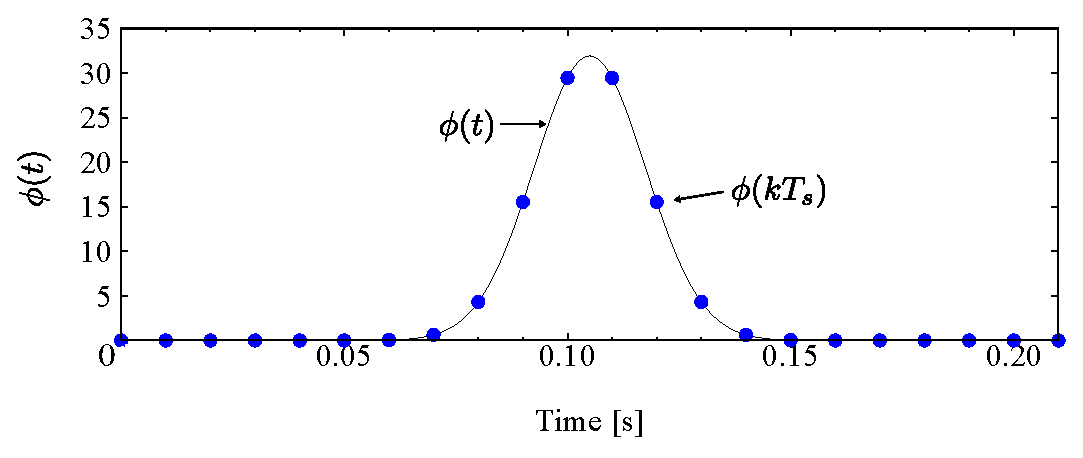
\includegraphics[width=0.8\linewidth]{phi.eps}\\
  (a) $\phi(k)$\\
\vspace{1.5cm}
\hspace{-17mm}
  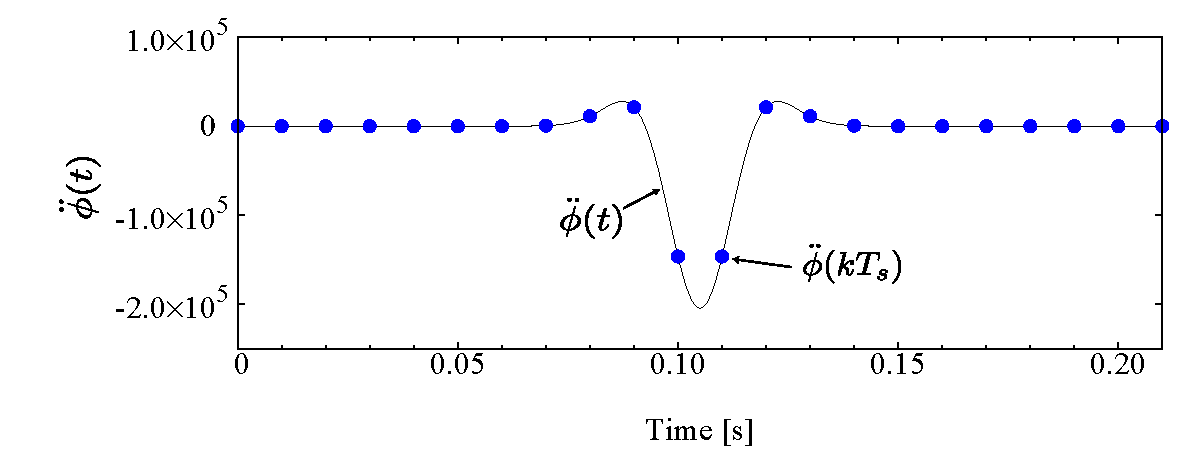
\includegraphics[width=0.9\linewidth]{ddphi.eps}\\
  (b) $\ddot{\phi}(k)$
 \end{center}
 \caption{超関数とその二階微分の概形($N=21$).}
 \label{ddphi}
\end{figure}


% \begin{figure}[htbp]
%     \centering
%         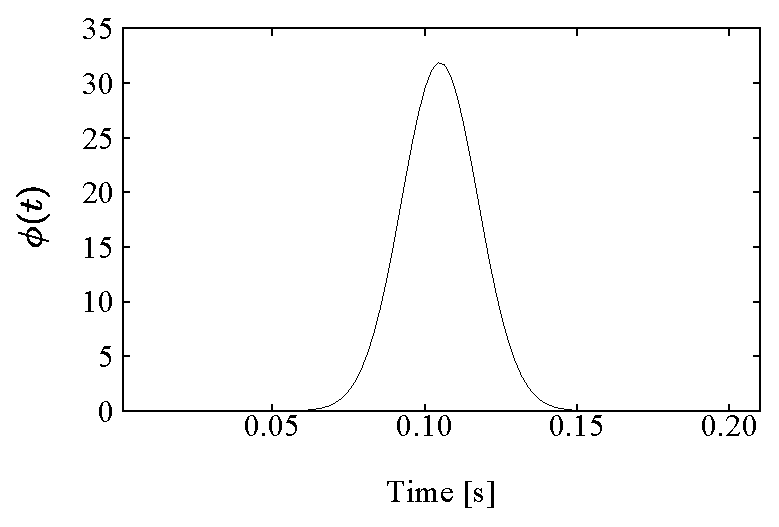
\includegraphics[scale=0.85]{phi0.01.eps}
%     \caption{$\phi(t)$の概形}
% 		\label{phi}
% \vspace{1.5cm}
%     \centering
%         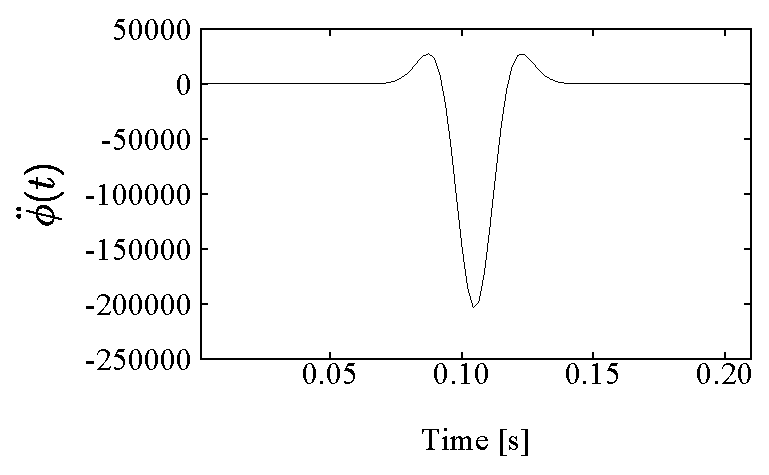
\includegraphics[scale=0.85]{ddphi0.01.eps}
%     \caption{$\ddot{\phi}(t)$の概形}
% 		\label{ddphi}
% \end{figure}

 \begin{figure}[h]
     \centering
  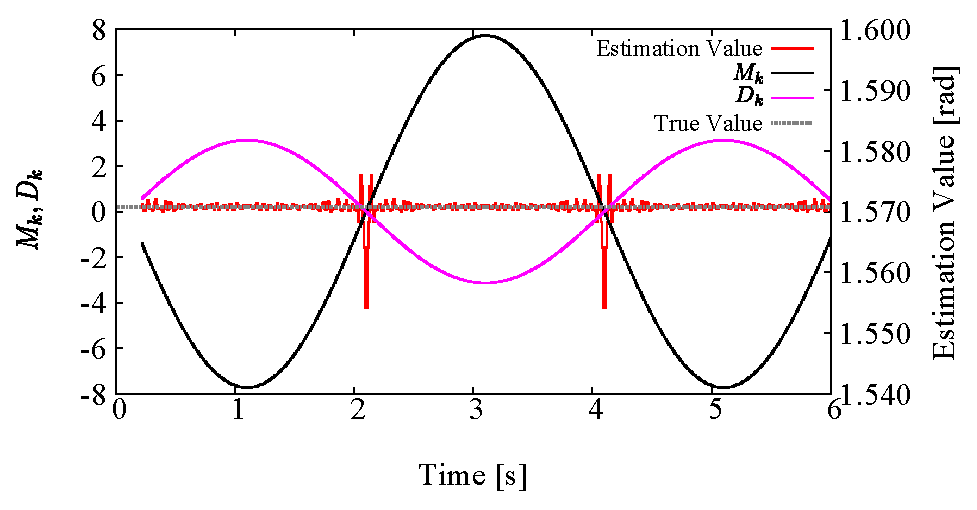
\includegraphics[scale=0.9]{check.eps}
 \caption{推定値と$M_k,D_k$}
 \label{check}
\end{figure}
さらに,それらを利用して推定した結果と推定値を算出するときの$M_k$,
$D_k$を図(\ref{check})に示す.ここで,$M_k$と$D_k$の交点に
注目し,その拡大したグラフを図\ref{checksinmini}に示す.図
\ref{checksinmini}より,$M_k$と$D_k$の交点付近では推定値が大きく振動
している.これは$D_k$が0に近づくにつれ,量子化誤差によって$M_k$と$D_k$の比が安定しなくなり,$\ddot{\phi}(t)$の値が増幅されるためである.
\begin{figure}[t]
 \centering
 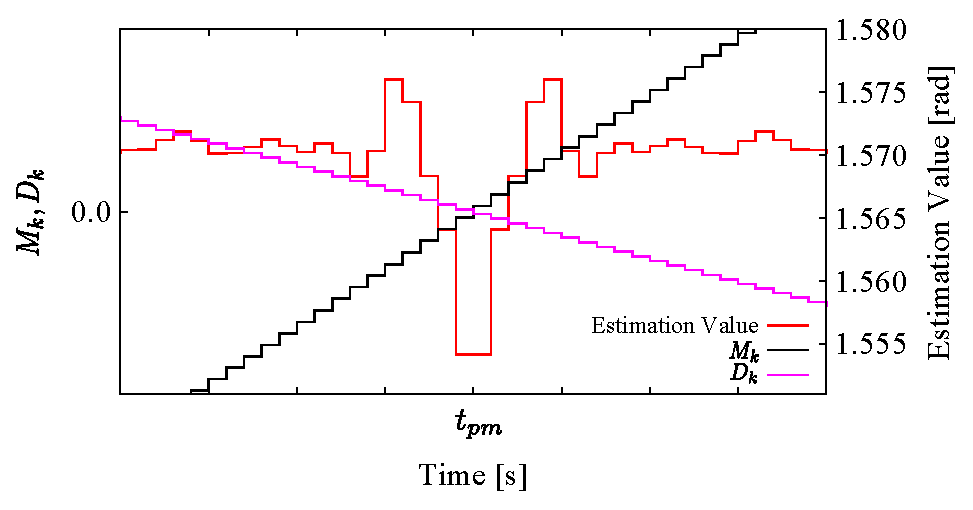
\includegraphics[scale=0.9]{checkzoom.eps}
    \caption{$M_k$と$D_k$の交点の拡大図と推定値}
		\label{checksinmini}
\end{figure}
\subsection{推定値の誤差の修正}
\subsubsection{量子化誤差の原因}
$M_k$と$D_k$の交点付近では,分母である$D_k$の値が小さくなることで推定値
が不安定となる.そこで,
推定値の誤差を修正するため,$M_k$と$D_k$の交点付近においては,ある一定個
数前の推定値を引き継ぐ処理を行う.推定誤差に影響している範囲は
ガウス関数のピーク値付近,すなわち$\phi(t)$,$\ddot{\phi}(t)$の
$\mu\pm3.3\sigma$の範囲である\cite{toukei}.そこで次式のように整数$W_x$を定める.

\begin{align}
 3.3\sigma \leq W_xT_s\label{3.3sigma}
\end{align}

ここで$W_x$は式(\ref{3.3sigma})を満たす最小の正の整数である.
\subsubsection{提案手法1}
誤差修正のため$M_k$の値の符号が反転した時刻から$W_x$個の推定値は採用しないとする.つまり時刻$t$の推定値
を$\hat{\omega}(t)$,符号が反転した時刻を$t_{pm}$とし,
$t=t_{pm}-(W_x+1)$のときの推定値を$\hat{\omega}_x$とすると,次式が成り立つ.
\begin{align}
 \hat{\omega}(t)=\hat{\omega}_x \hspace{1cm} ( t_{pm}\leq t \leq t_{pm}+W_xT_s )\label{omegahat}
\end{align}
これらを図\ref{checkexp}に図示する.
式(\ref{3.3sigma}),(\ref{omegahat})を用いてシミュレーションにおける推定誤
差を修正する.シミュレーションでは式(\ref{19})より
$\sigma=0.0128$であるので,式(\ref{3.3sigma})より,$W_x=5$となる.式
(\ref{omegahat})より,推定誤差を修正したときの推定値を図
\ref{checkmod1exp}に示す.
以上より,$M_k$と$D_k$の交点付近の推定誤差の半分を修正することができた.
提案手法1の欠点は,$M_k$の値の符号が反転した時刻から$W_xT_s$前の推定誤差
は残ってしまう点である.また,利点としては,リアルタイムに推定値が得られる点である.
\begin{figure}[htbp]
 \centering
 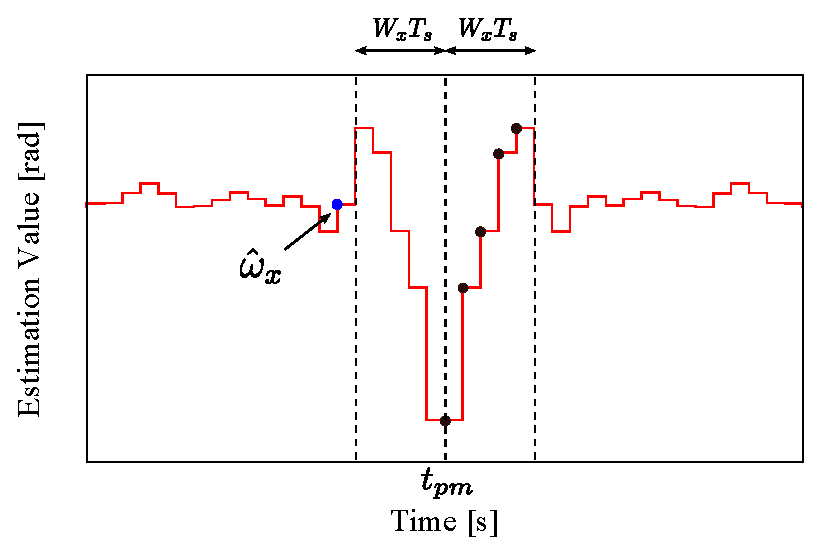
\includegraphics[scale=0.9]{checkzoomexp.eps}
  \hspace{105mm}
    \caption{シミュレーションにおける$W_xT_s$,$t_{pm}$,$\hat{\omega}_x$}
		\label{checkexp}
 \end{figure}
\vspace{1cm}
 \begin{figure}[htbp]
 \centering
 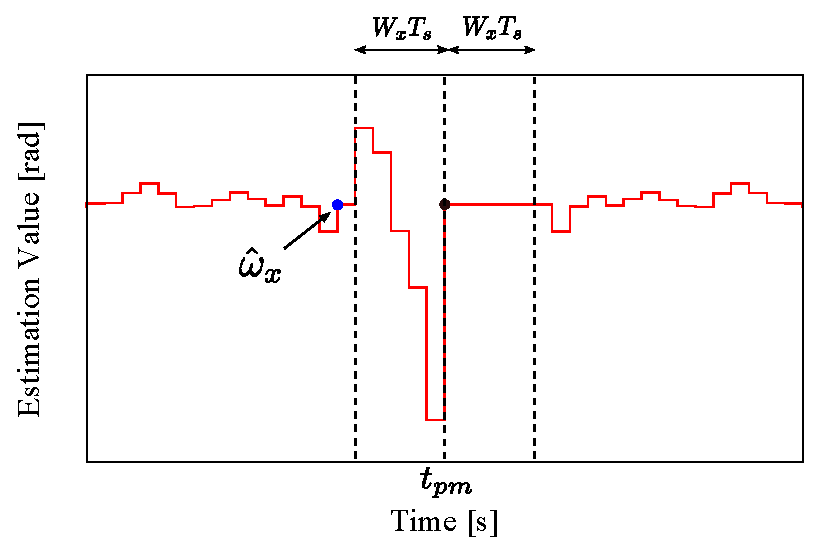
\includegraphics[scale=0.9]{checkmod1exp.eps}
 \hspace{103mm}
    \caption{提案手法1による誤差修正後の$M_k$と$D_k$の交点の拡大図}
		\label{checkmod1exp}
\end{figure}
\clearpage
\subsubsection{提案手法2}
誤差修正のため$M_k$の値の符号が反転した時刻から前後$W_x$個の推定値は採用
しないとする.つまり$\hat{\omega}(t)$,$t_{pm}$,$\hat{\omega}_x$を提案
手法1と同様に定義すると,次式が成り立つ.
\begin{align}
 \hat{\omega}(t)=\hat{\omega}_x \hspace{1cm} ( t_{pm}-(W_x+1)T_s \leq t
 \leq t_{pm}+W_xT_s )
\label{omegahat2}
\end{align}

式(\ref{omegahat2})より,推定誤差を修正したときの推定値を図
\ref{checkmod2exp}に示す.
以上より,$M_k$と$D_k$の交点付近の推定誤差を修正することができた.
提案手法2の欠点は,$M_k$の値の符号が反転した時刻から$W_xT_s$前の推定値を
更新せねばならず,その時間だけ推定結果が得るのが遅れる点である.また,利
点としては,提案手法1では残ってしまう時刻$t_{pm}$より前の誤差が修正できる点である.

 \begin{figure}[h]
 \centering
 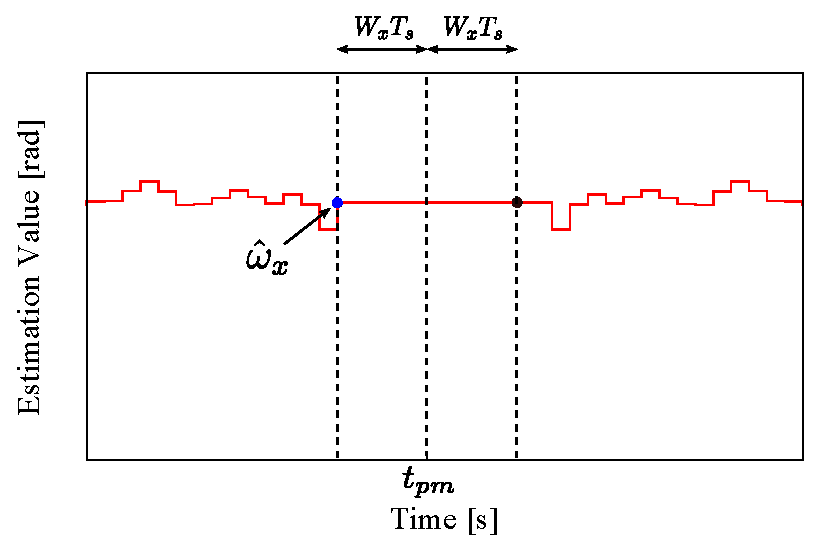
\includegraphics[scale=0.9]{checkmod2exp.eps}
 \hspace{103mm}
    \caption{提案手法2による誤差修正後の$M_k$と$D_k$の交点の拡大図}
		\label{checkmod2exp}
\end{figure}


\section{実験}

\subsection{実験装置}
実験では図\ref{fig:system}(a)に示すような単振子を用いる.振子の先端部
に図\ref{fig:system}(b)に示すようなATP-Promotions社製
の小型多機能センサ[型番:TSND121]を取り付け,これによって計測された角速度
データを式(\ref{1})の$x(t)$として周波数推定に利用する.この
センサは三軸方向別に角速度データ得られ,サンプリングインターバルは1[s]〜255[s]で
変更でき,分解能は0.08[dps]である.実験では振子の単振動の振幅方向を軸と
した角速度データ使用する.
得られた角速度データはBluetooth通信でPCに送信される.\\

\begin{figure}[htbp]
  \begin{center}
    \begin{tabular}{c}

 \begin{minipage}{0.5\hsize}
  \begin{center}
   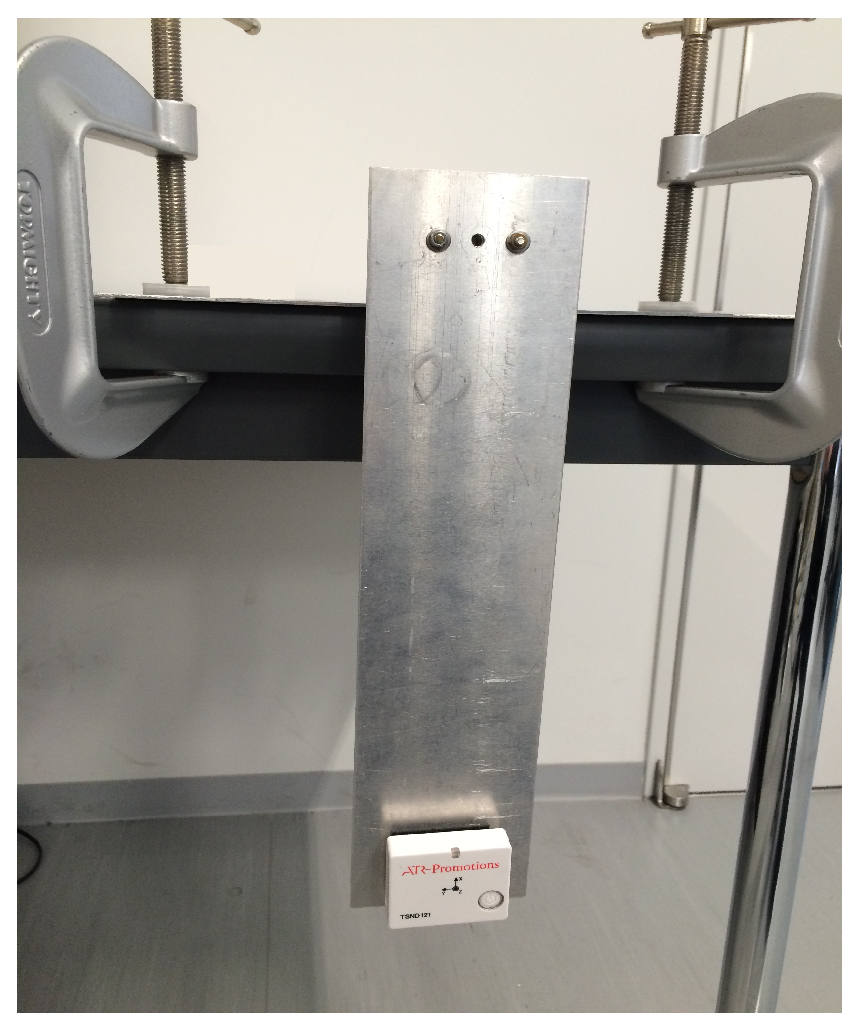
\includegraphics[width=70mm]{furiko.eps}
		\hspace{10mm}  \subfigure(a)振り子 
 \end{center}
  \label{furiko}
 \end{minipage}
 \begin{minipage}{0.5\hsize}
  \begin{center}
   \includegraphics[width=86mm]{sensor.eps}
	\hspace{10mm} \subfigure(b)角速度センサ 
 \end{center}
  \label{sensor}
 \end{minipage}

 \end{tabular}
    \caption{実験装置}
    \label{fig:system}
  \end{center}
\end{figure}

\newpage
\subsection{実験方法}
\begin{enumerate}
\item 角速度センサのサンプリング周期を50[Hz]に設定する.
\item 単振子の振子部分を手で持ち上げ,静かに離して振子を振る.
\item 角速度データの取得を開始する.
\item 10周期程度の角速度データが得られた時点でデータの取得を停止する.
\item 第\ref{sec:distributions}節と第\ref{sec:simulation}節で述べた手法により振り子の単振動の角速度データから周波数を推定する.
\end{enumerate}

\subsection{実験結果と考察}
図\ref{check50}に量子化ノイズがある場合の推定結果を,図\ref{check50only}に
その推定値のみを,図\ref{check50mod1}に提案手法1を用いた推定値を,
図\ref{check50}に提案手法2を用いた推定値を示す.シミュレーションと比較すると,推
定値が振動していることがわかる.また,量子化誤差修正後も推定値が振動して
いる時間があるのがわかる.これは実験装置の振動や,離散化された角速
度データの量子化誤差が原因であると考えられる.また,
$t_{pm}$の$W_xT_s$前の時刻の推定値$\hat{\omega}_{x}$に誤差がある場合,誤
差を持つ推定値が引き継がれるため,$W_x$を大きく設定する必要がある.
\vspace{3cm}
\begin{figure}[htbp]
 \centering
 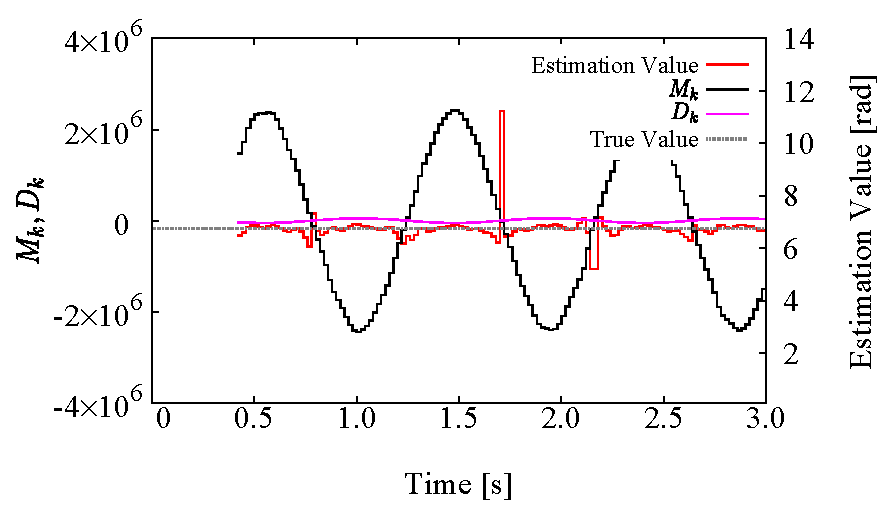
\includegraphics[scale=0.9]{check50.eps}
    \caption{実験による推定値と$M_k$と$D_k$}
		\label{check50}
\end{figure}
\begin{figure}[htbp]
 \centering
 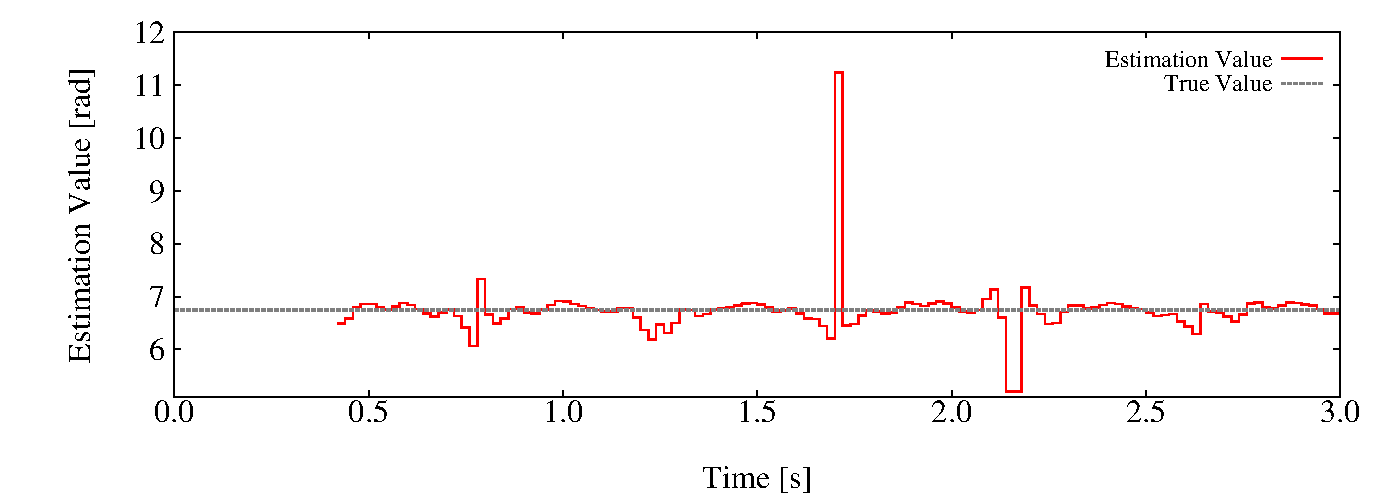
\includegraphics[scale=0.7]{check50only.eps}
    \caption{実験による推定値}
		\label{check50only}
\end{figure}
\begin{figure}[htbp]
 \centering
 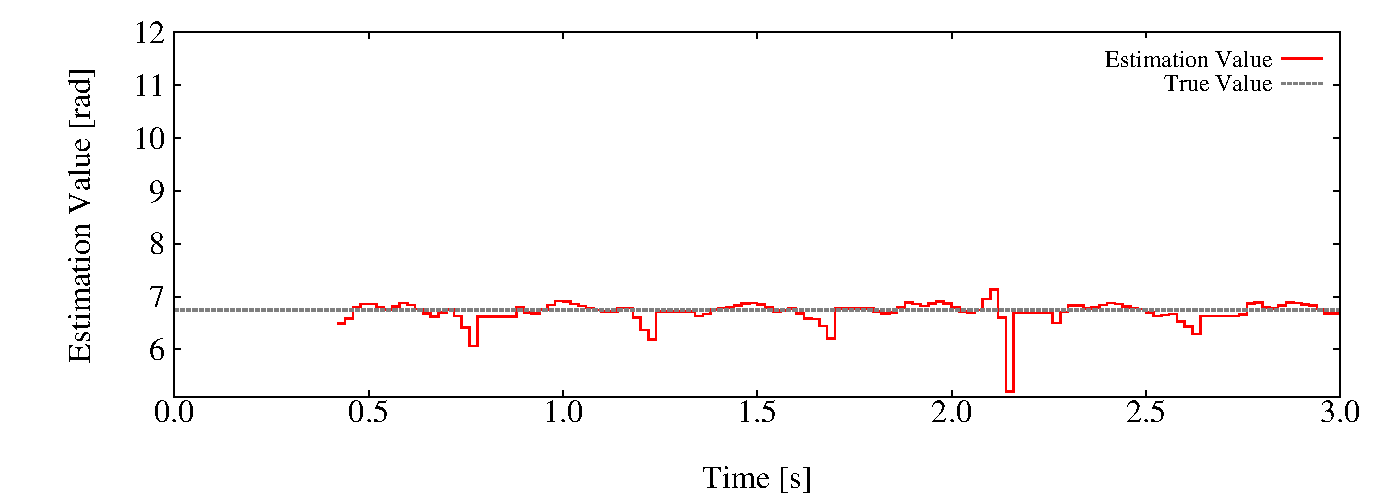
\includegraphics[scale=0.7]{check50mod1.eps}
    \caption{提案手法1を用いた実験による推定値}
		\label{check50mod1}
\end{figure}\begin{figure}[htbp]
 \centering
 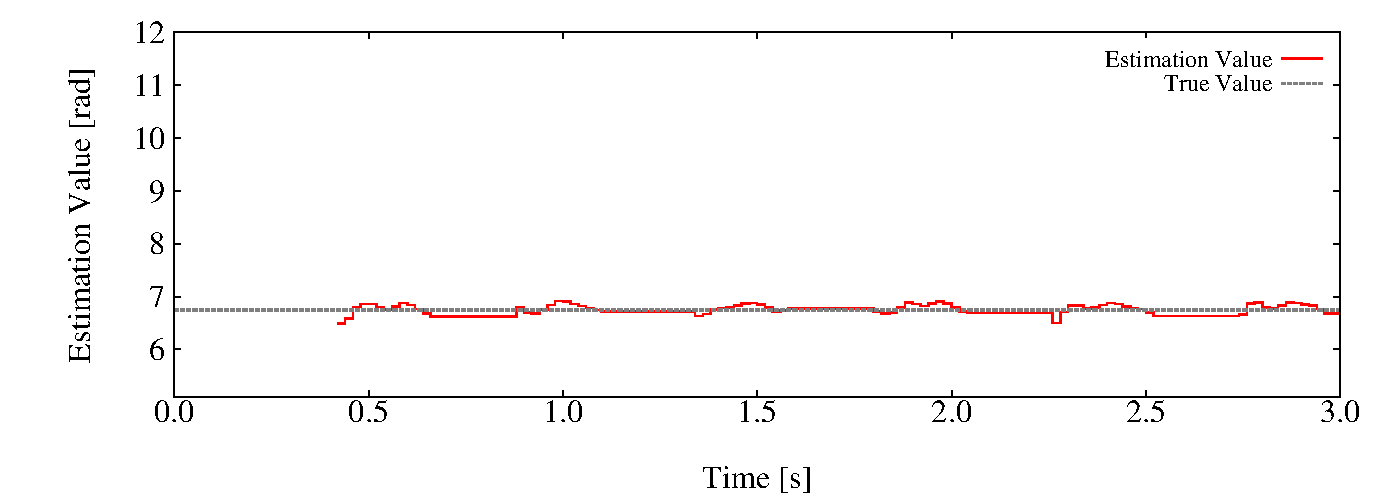
\includegraphics[scale=0.7]{check50mod2.eps}
		\caption{提案手法2を用いた実験による推定値}
		\label{check50mod2}
\end{figure}

% \ref{062045_7Feb15}で述べた手法により単振子の振動の角速度データから周波
% 数を推定する.推定する振動の1周期に対して,推定に利用するデータの範囲が
% 占める割合と本手法の推定精度の関係を実験結果から検証する.
% ここで式(\ref{11})の$\sigma$は$T_s$, $N$に従属する変数として定めるため,
% 以下のような関数を定め,式(\ref{(19)})を満たすように設定した.
% \begin{align}
%  \sigma=((N-20)/2+20)T_s/16
% \end{align}
% 以下図(\ref{075105_6Feb15})〜図(\ref{075122_6Feb15})に取得した角速度データと推定結果を示
% す.推定結果にはノイズ低減のため,シミュレーションと同様に
% 推定値に11個のデータを参考とする中央値フィルタをかけた.
% 次の公式を用いて周波数$\omega$を算出し,真値とした.$T$[s]は1周期の時間とする.
% \begin{align}
%  \omega=2\pi/T \label{23}
% \end{align}
% \begin{figure}[htbp]
%     \centering
%         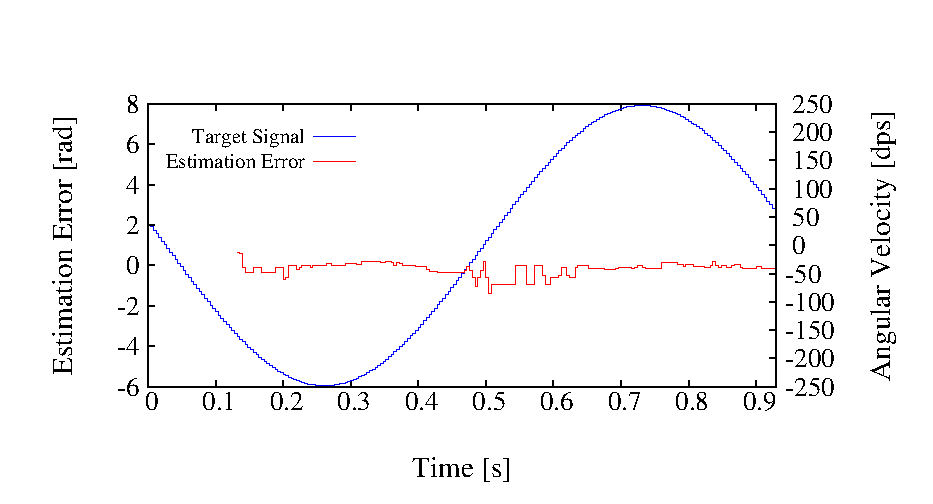
\includegraphics[scale=0.85]{250_10.eps}
%     \caption{250[Hz],1/10周期}
% 		\label{075105_6Feb15}
% \vspace{0.5cm}
%         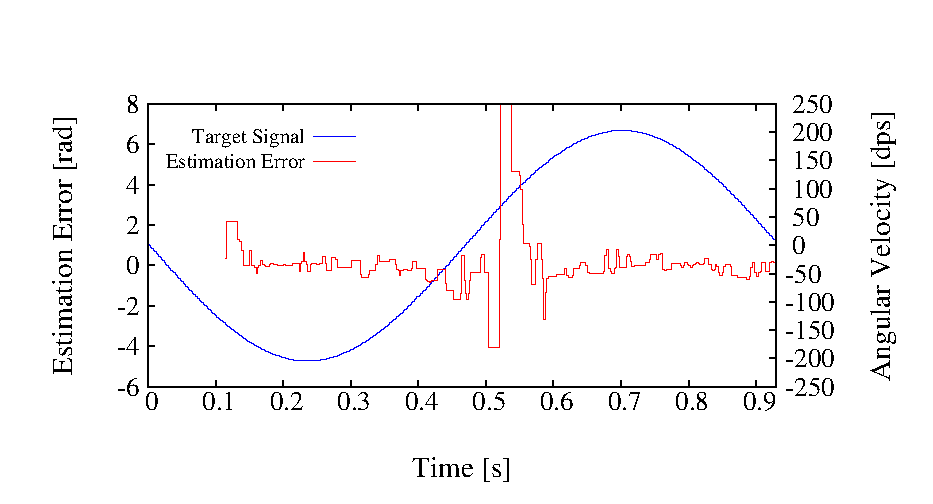
\includegraphics[scale=0.85]{500_10.eps}
%     \caption{500[Hz],1/10周期}
% \vspace{0.5cm}
%         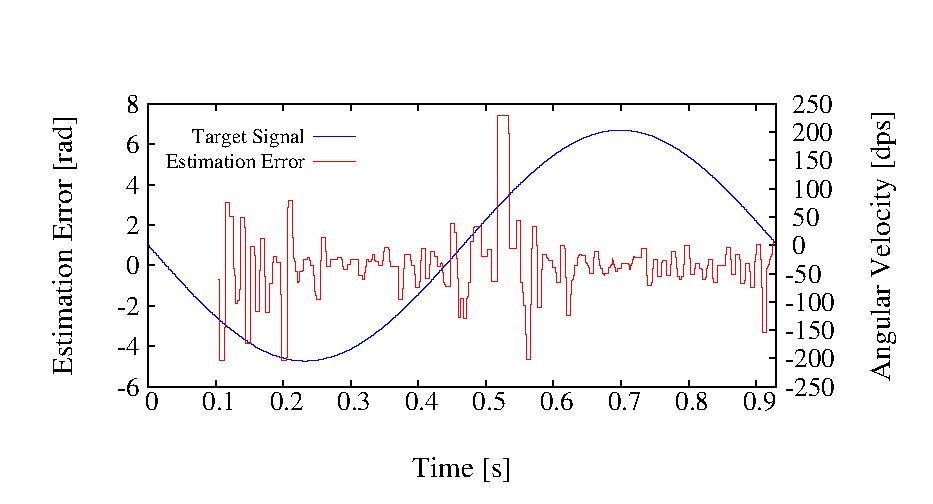
\includegraphics[scale=0.85]{1000_10.eps}
%     \caption{1000[Hz],1/10周期}
% \end{figure}
% \begin{figure}[htbp]
%     \centering
%         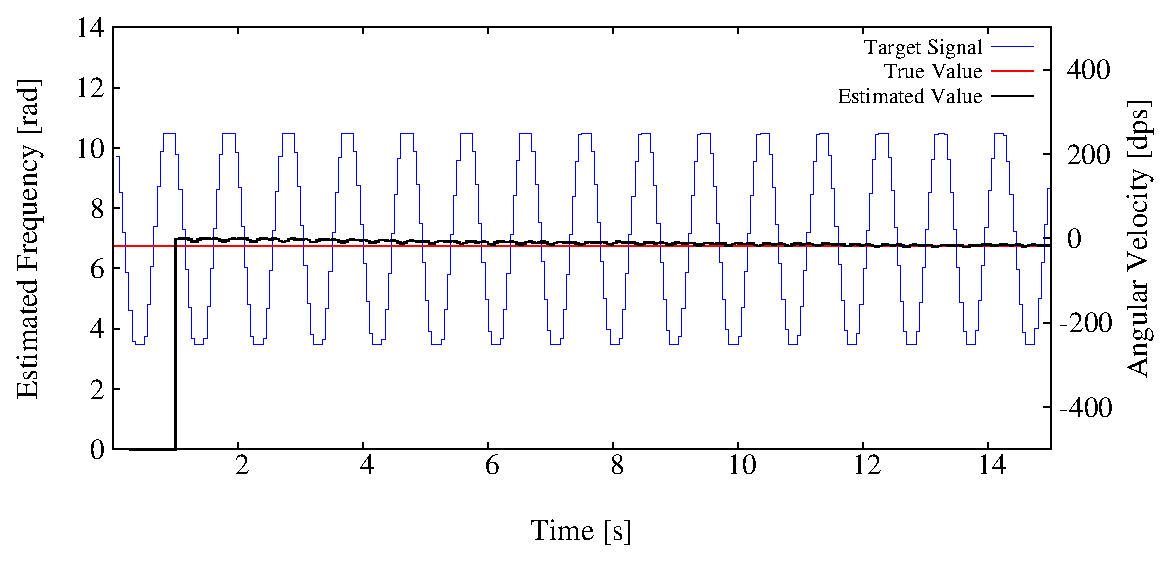
\includegraphics[scale=0.72]{20hz20.eps}
%     \caption{20Hz, N=20}
% 		\label{075105_6Feb15}
% \vspace{0.5cm}
%         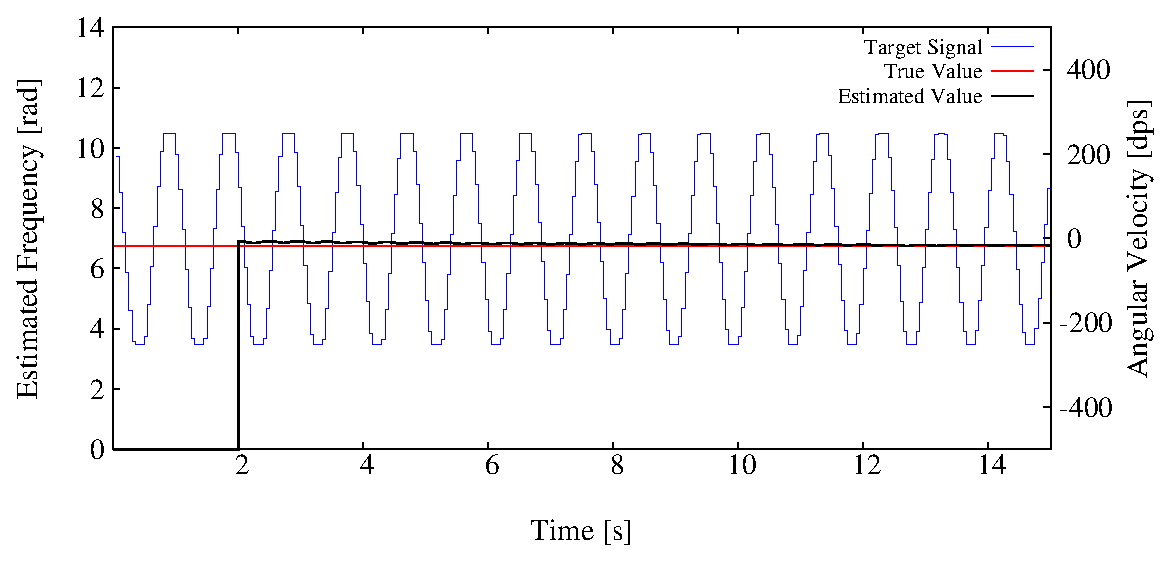
\includegraphics[scale=0.72]{20hz40.eps}
%     \caption{20Hz, N=40}
% \vspace{0.5cm}
%         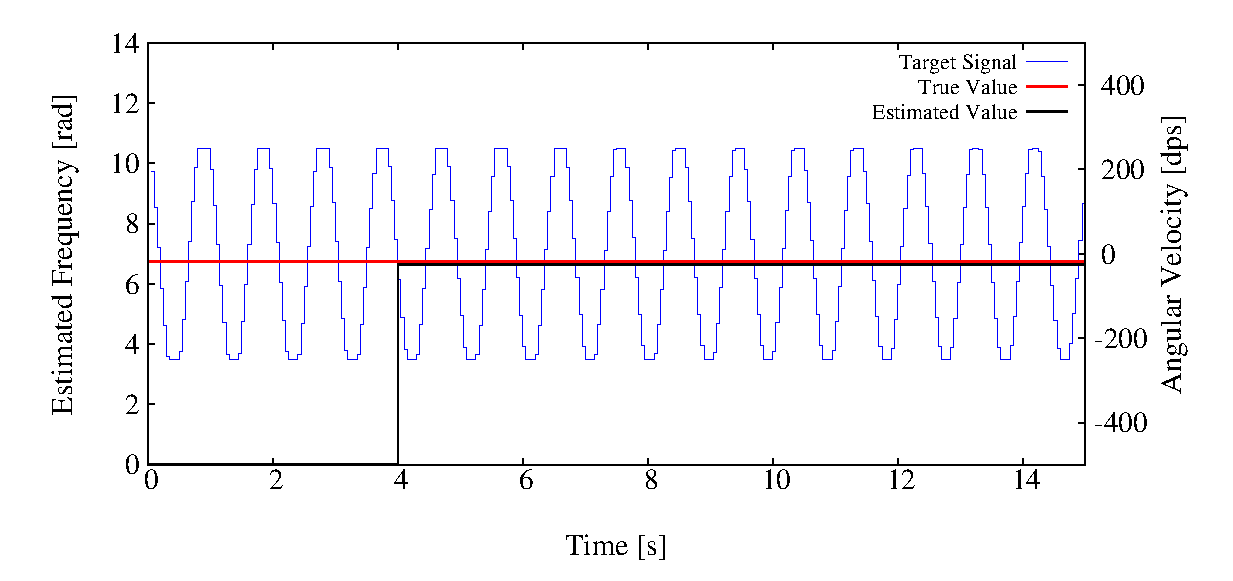
\includegraphics[scale=0.72]{20hz80.eps}
%     \caption{20Hz, N=80}
% \end{figure}
% \begin{figure}[htbp]
%     \centering
%         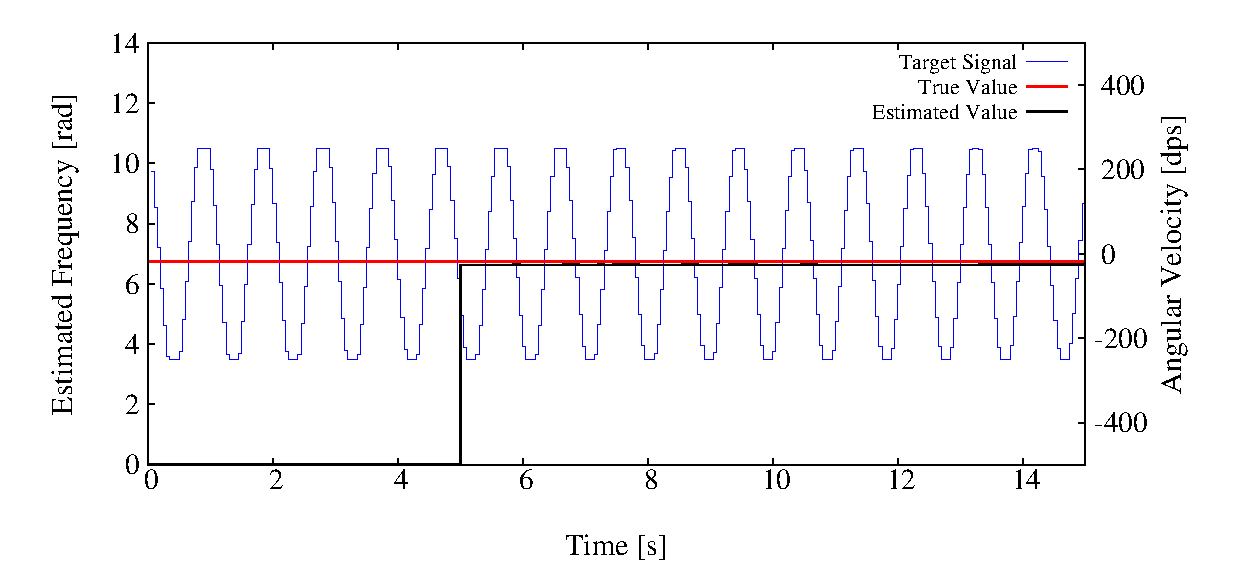
\includegraphics[scale=0.72]{20hz100.eps}
%     \caption{20Hz, N=100}
% \vspace{0.5cm}
%         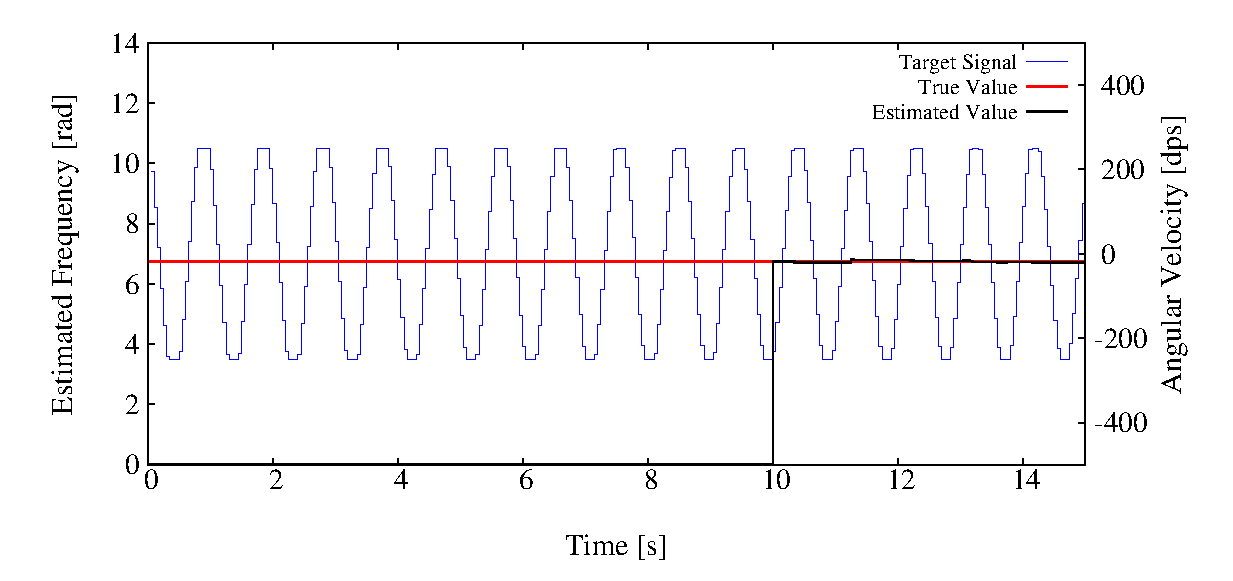
\includegraphics[scale=0.72]{20hz200.eps}
%     \caption{20Hz, N=200}
% \vspace{0.5cm}
%         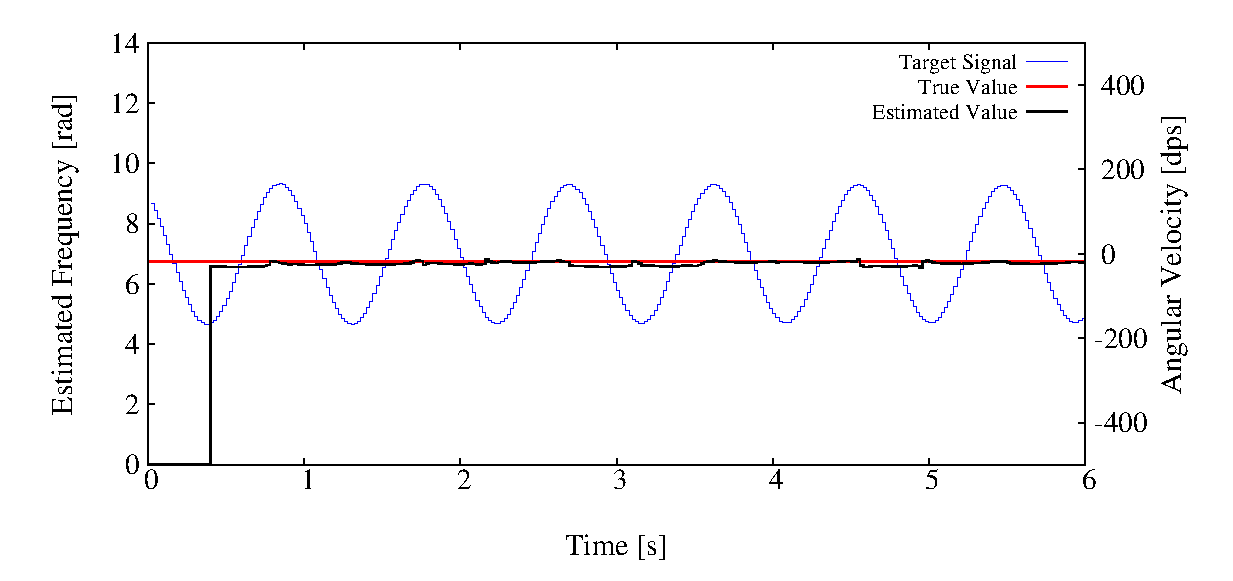
\includegraphics[scale=0.72]{50hz20.eps}
%     \caption{50Hz, N=20}
% \end{figure}
% \begin{figure}[htbp]
%     \centering
%         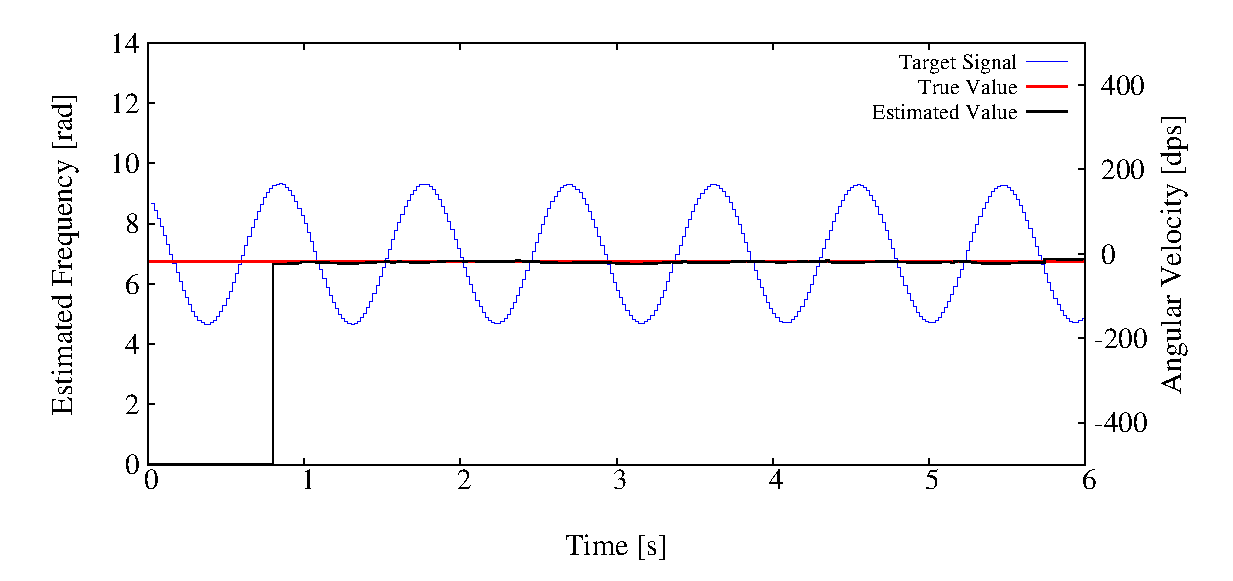
\includegraphics[scale=0.72]{50hz40.eps}
%     \caption{50Hz, N=40}
% \vspace{0.5cm}
%         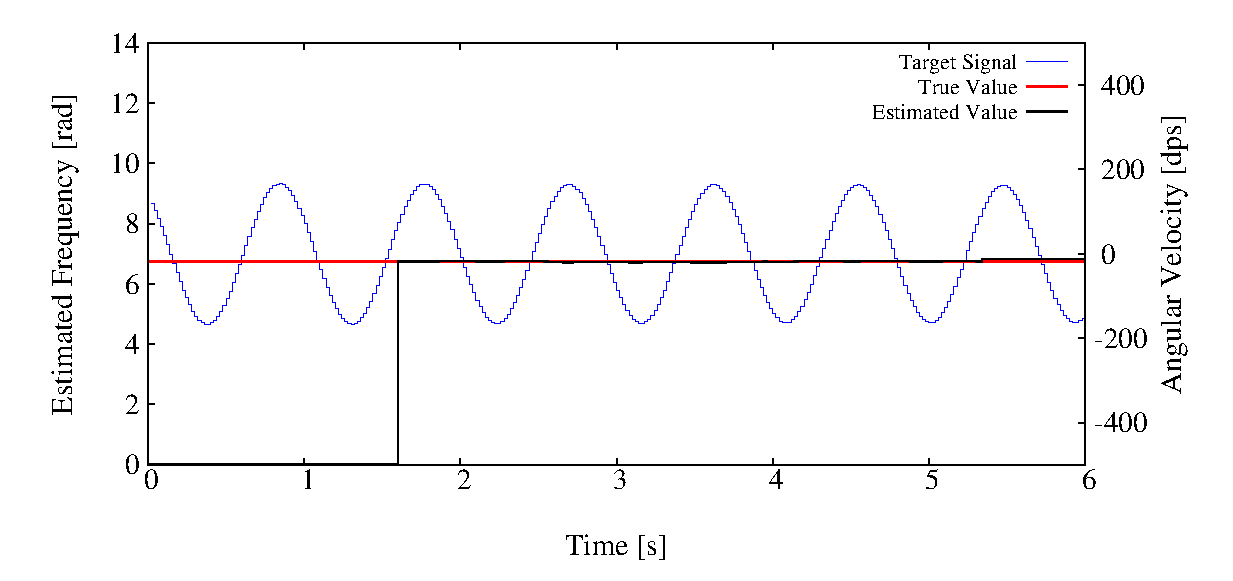
\includegraphics[scale=0.72]{50hz80.eps}
%     \caption{50Hz, N=80}
% \vspace{0.5cm}
%         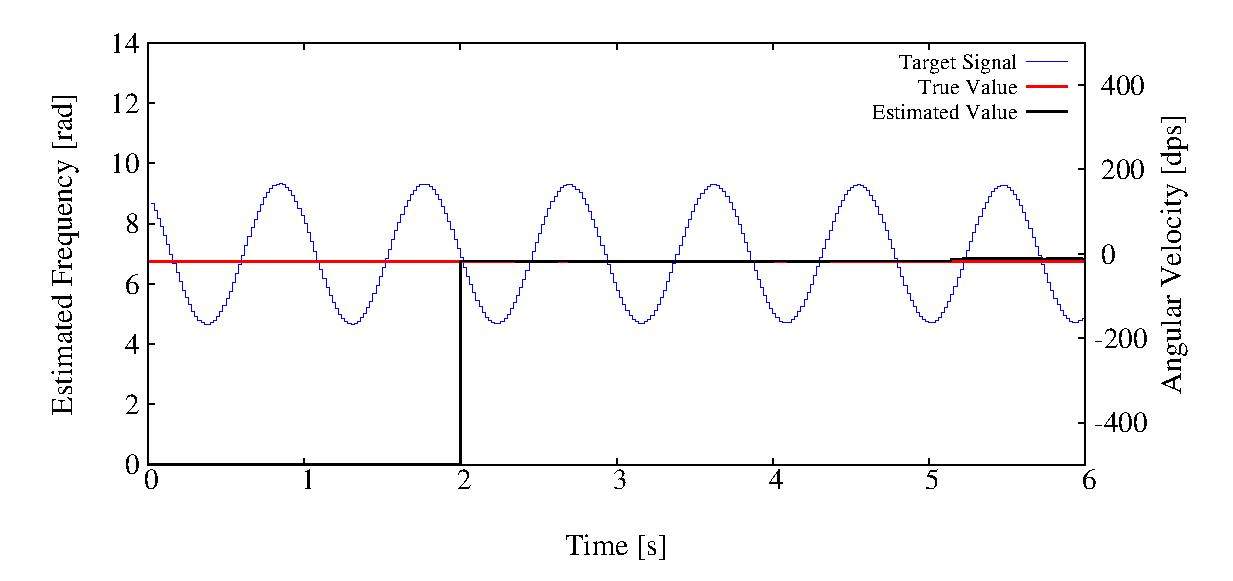
\includegraphics[scale=0.72]{50hz100.eps}
%     \caption{50Hz, N=100}
% \end{figure}
% \begin{figure}[htbp]
%     \centering
%         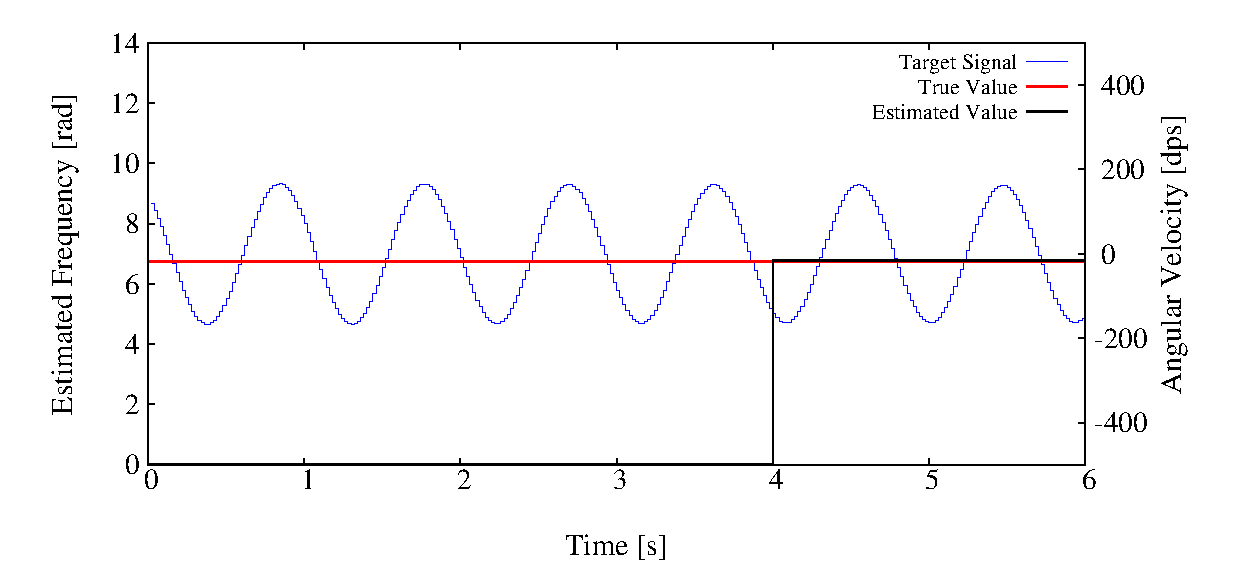
\includegraphics[scale=0.72]{50hz200.eps}
%     \caption{50Hz, N=200}
% \vspace{0.5cm}
%         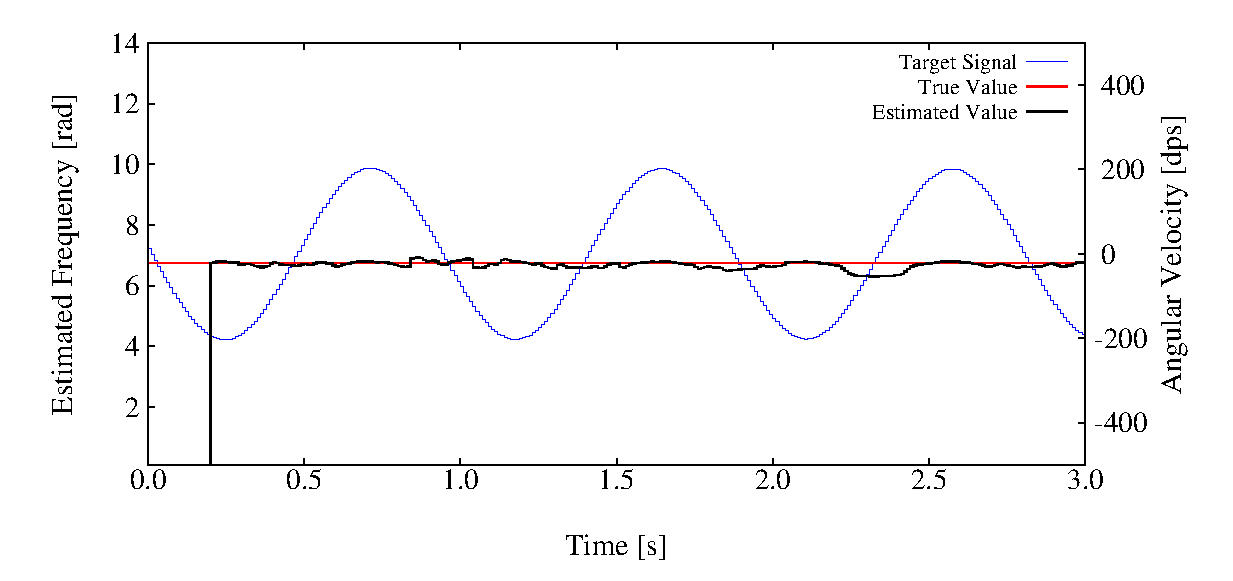
\includegraphics[scale=0.72]{100hz20.eps}
%     \caption{100Hz, N=20}
% \vspace{0.5cm}
%         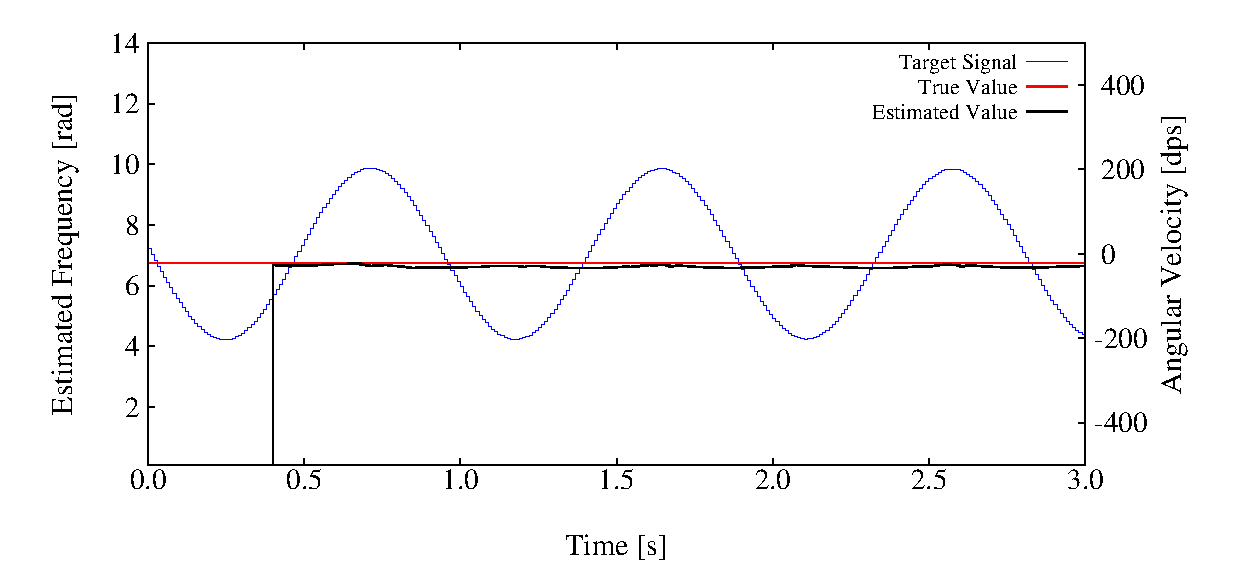
\includegraphics[scale=0.72]{100hz40.eps}
%     \caption{100Hz, N=40}
% \end{figure}
% \begin{figure}[htbp]
%     \centering
%         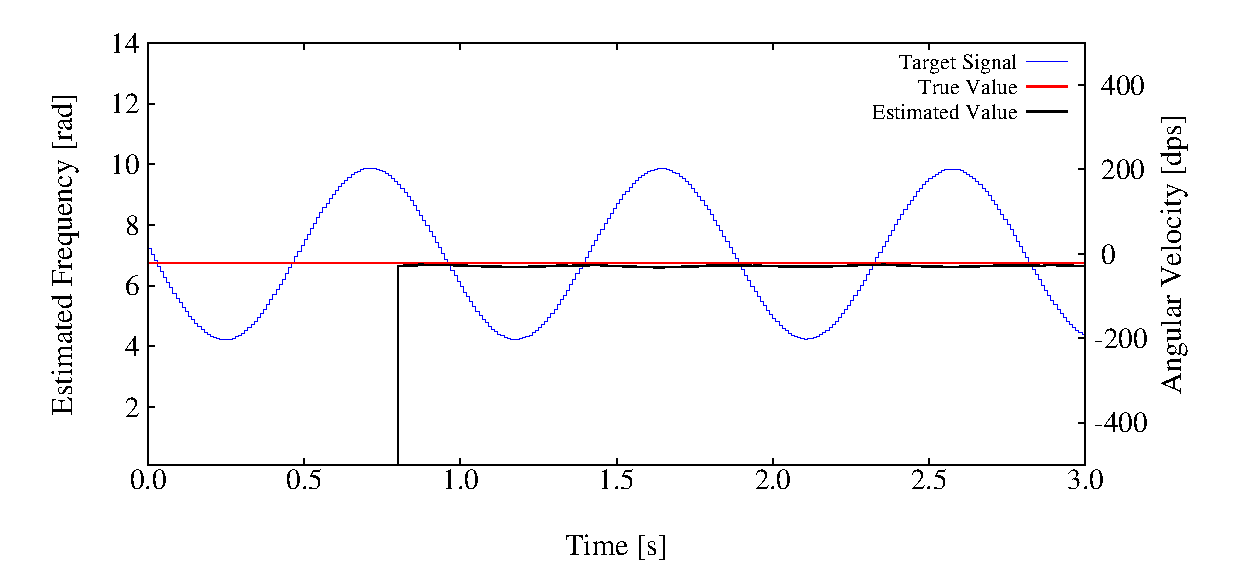
\includegraphics[scale=0.72]{100hz80.eps}
%     \caption{100Hz, N=80}
% \vspace{0.5cm}
%         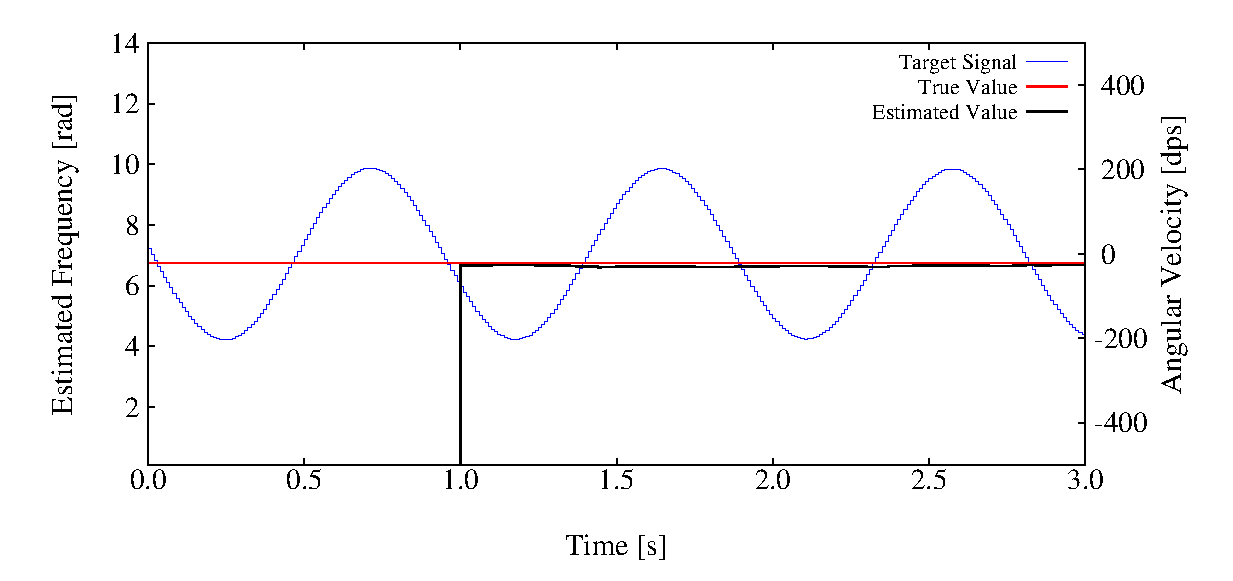
\includegraphics[scale=0.72]{100hz100.eps}
%     \caption{100Hz, N=100}
% \vspace{0.5cm}
%         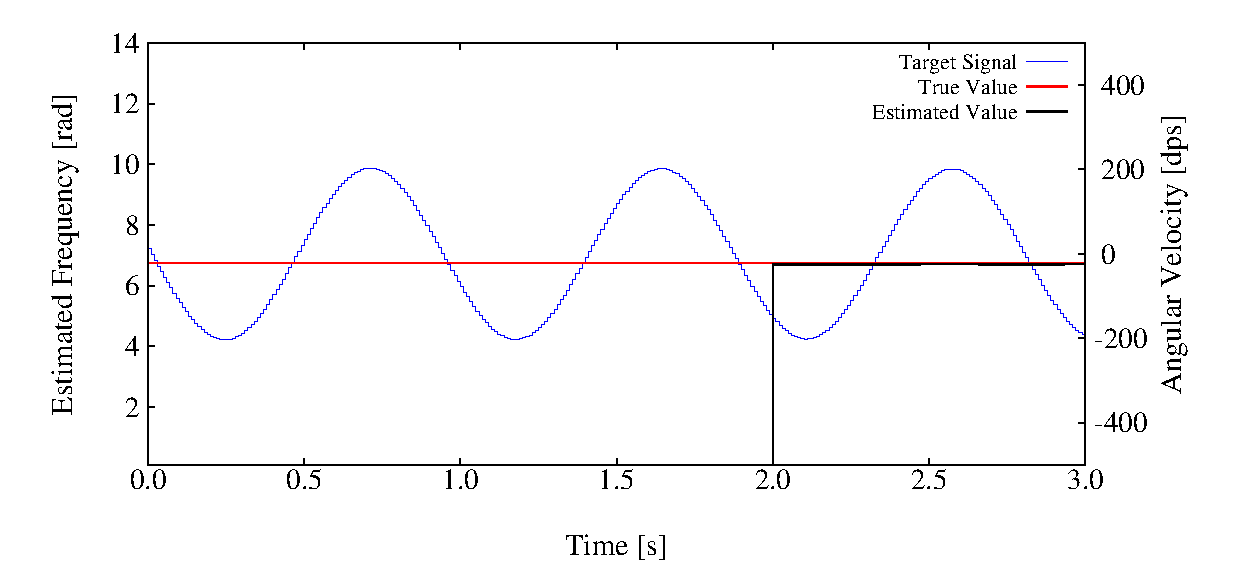
\includegraphics[scale=0.72]{100hz200.eps}
%     \caption{100Hz, N=200}
% \end{figure}
% \begin{figure}[htbp]
%     \centering
%         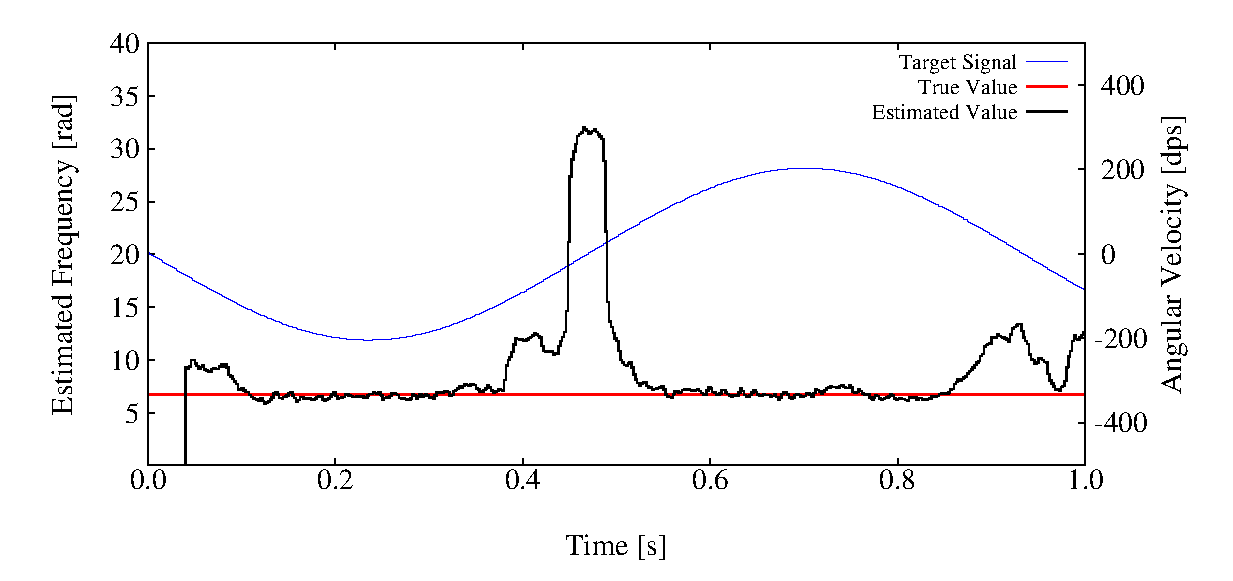
\includegraphics[scale=0.72]{500hz20.eps}
%     \caption{500Hz, N=20}
% \vspace{0.5cm}
%         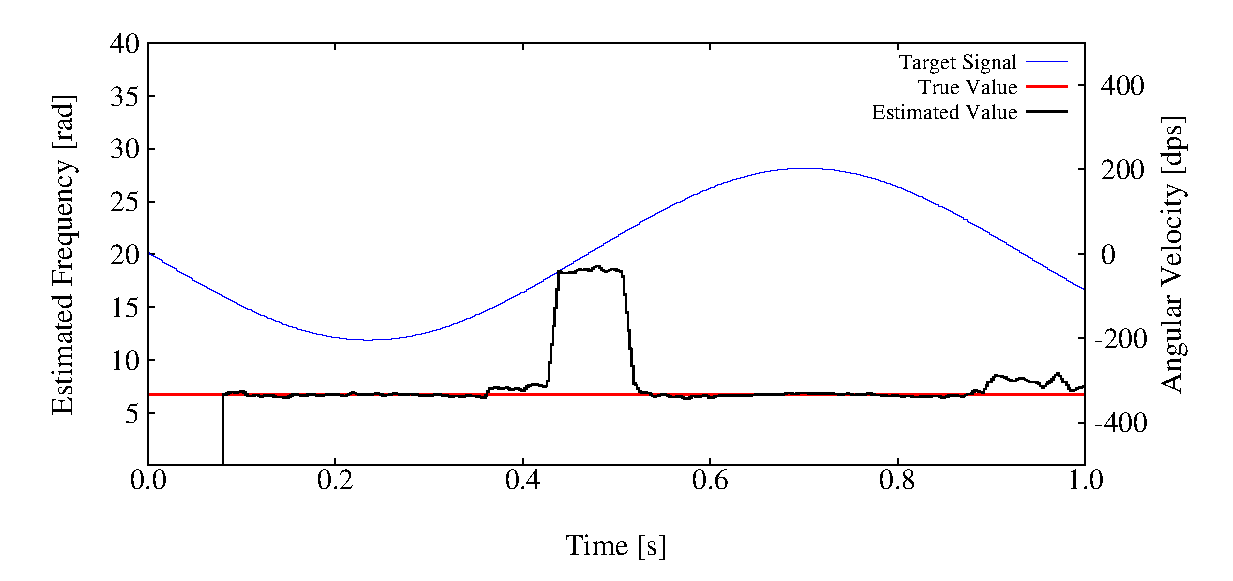
\includegraphics[scale=0.72]{500hz40.eps}
%     \caption{500Hz, N=40}
% 		\label{020210_7Feb15}
% \vspace{0.5cm}
%         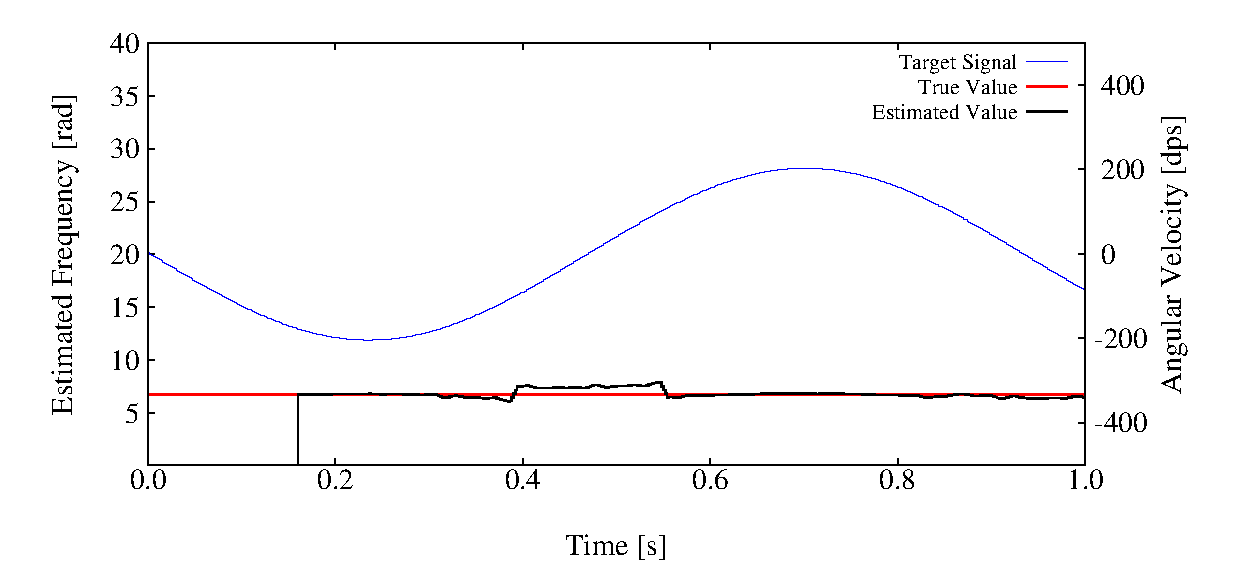
\includegraphics[scale=0.72]{500hz80.eps}
%     \caption{500Hz, N=80}
% \end{figure}
% \begin{figure}[htbp]
%     \centering
%         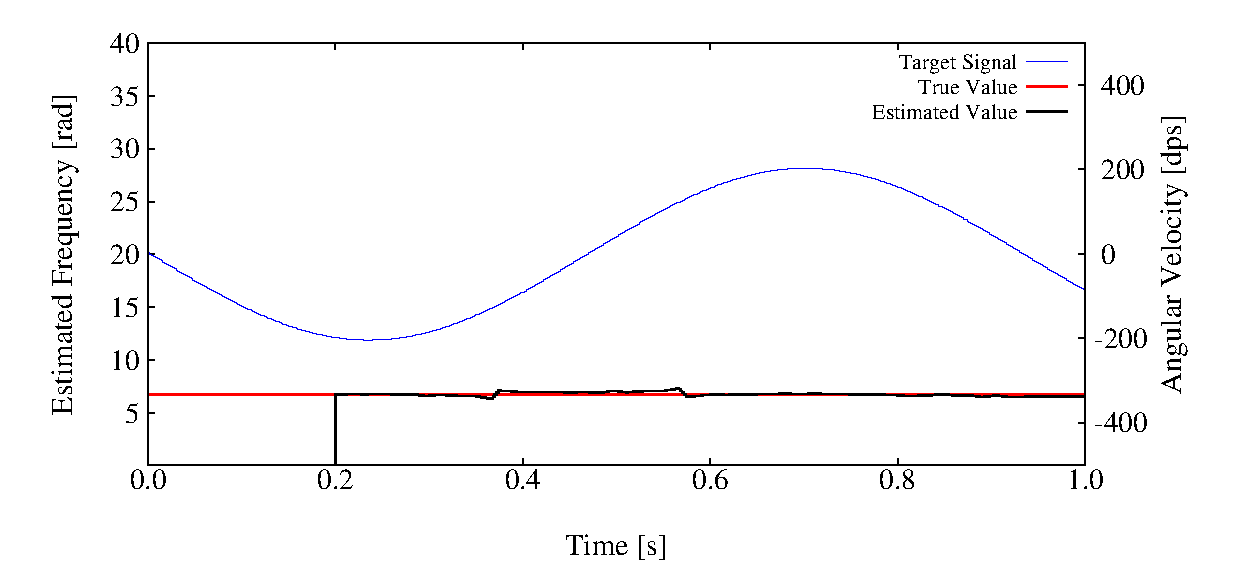
\includegraphics[scale=0.72]{500hz100.eps}
%     \caption{500Hz, N=100}
% \vspace{0.5cm}
%         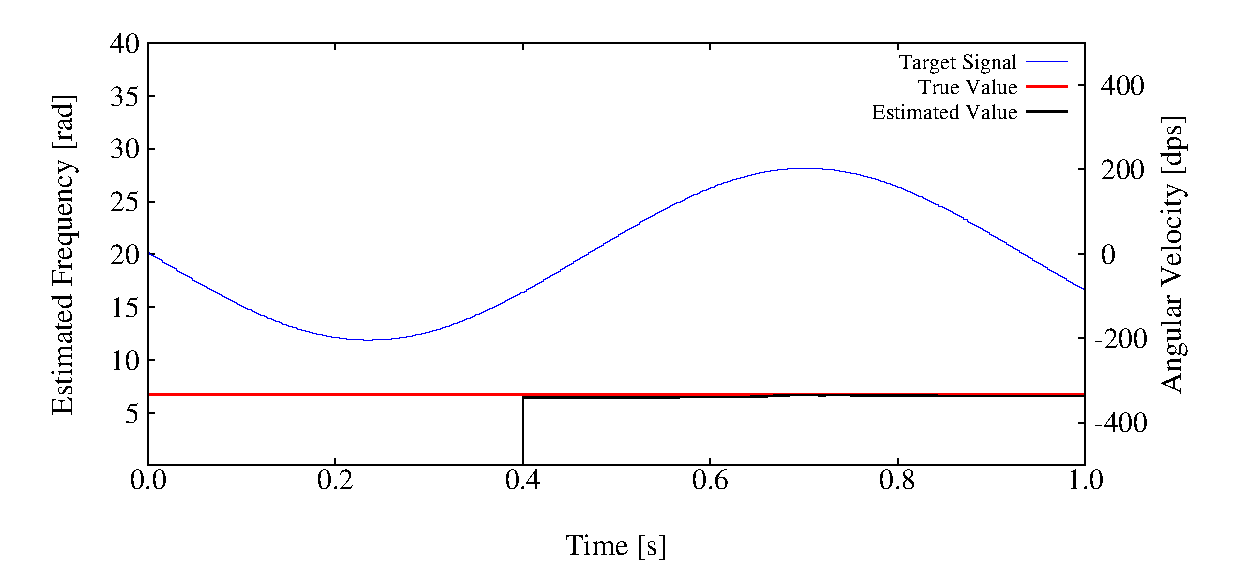
\includegraphics[scale=0.72]{500hz200.eps}
%     \caption{500Hz, N=200}
% \vspace{0.5cm}
%         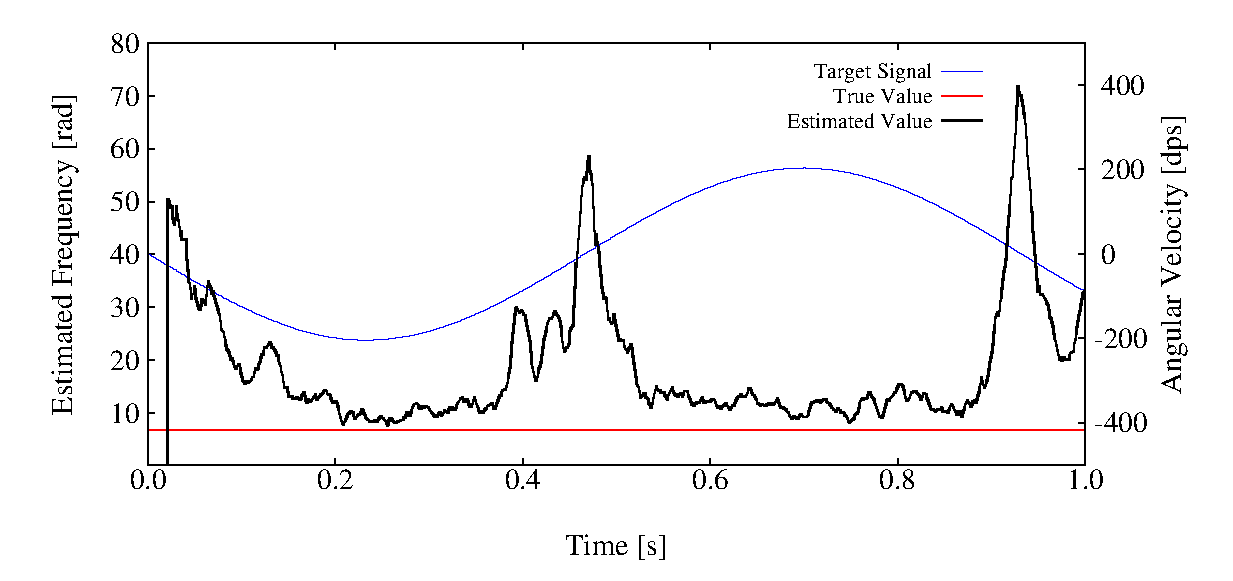
\includegraphics[scale=0.72]{1000hz20.eps}
%     \caption{1000Hz, N=20}
% \end{figure}
% \begin{figure}[htbp]
%     \centering
%         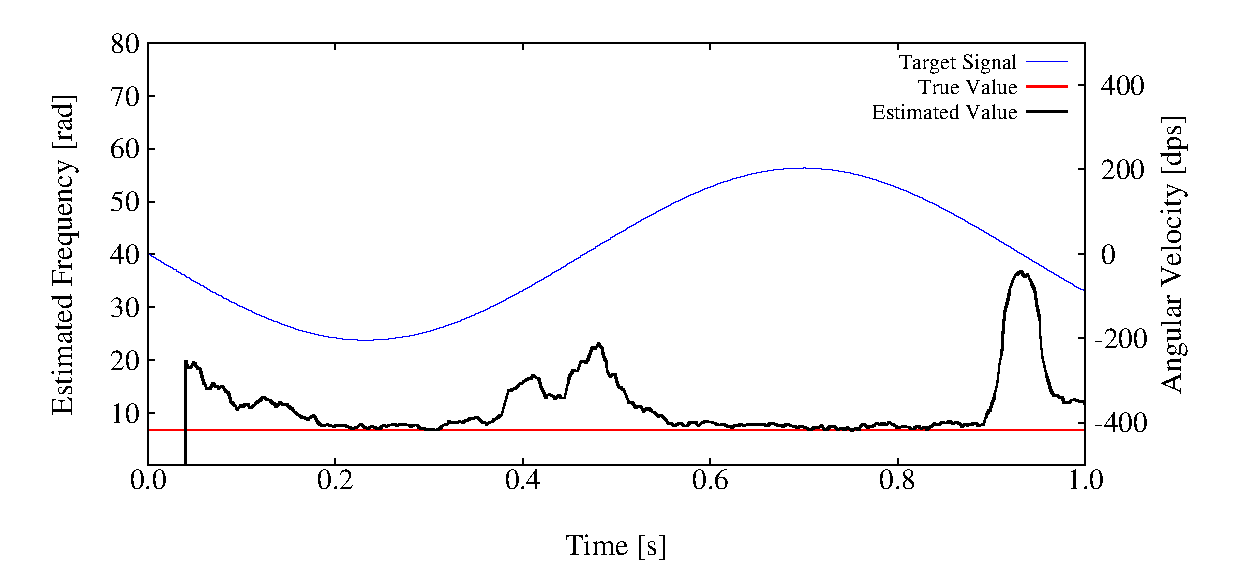
\includegraphics[scale=0.72]{1000hz40.eps}
%     \caption{1000Hz, N=40}
% \vspace{0.5cm}
%         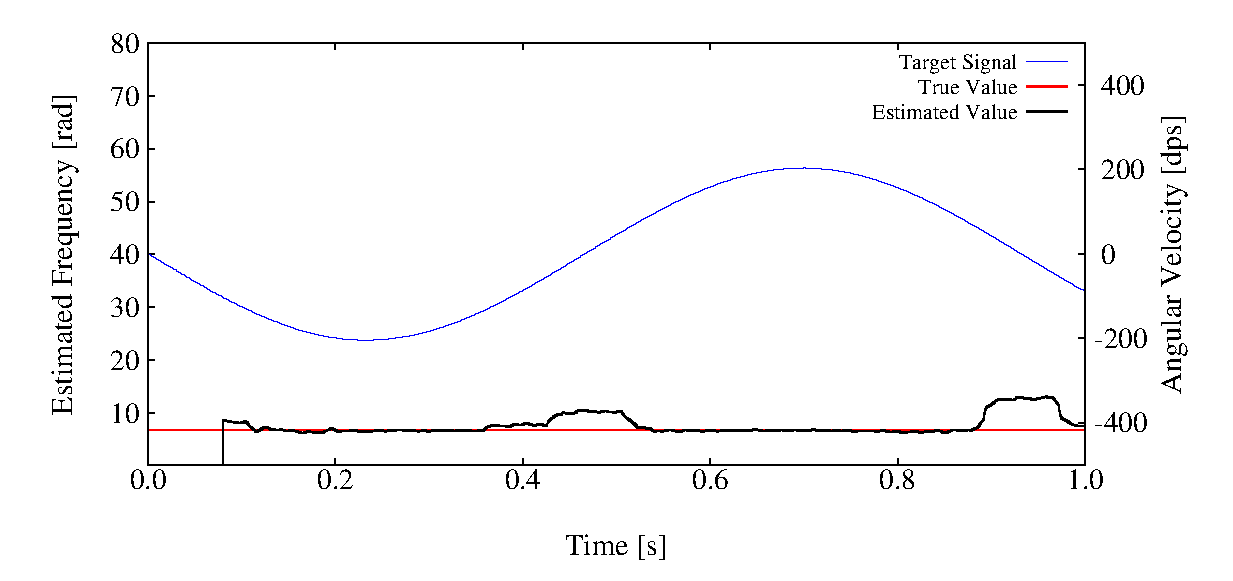
\includegraphics[scale=0.72]{1000hz80.eps}
%     \caption{1000Hz, N=80}
% \vspace{0.5cm}
%         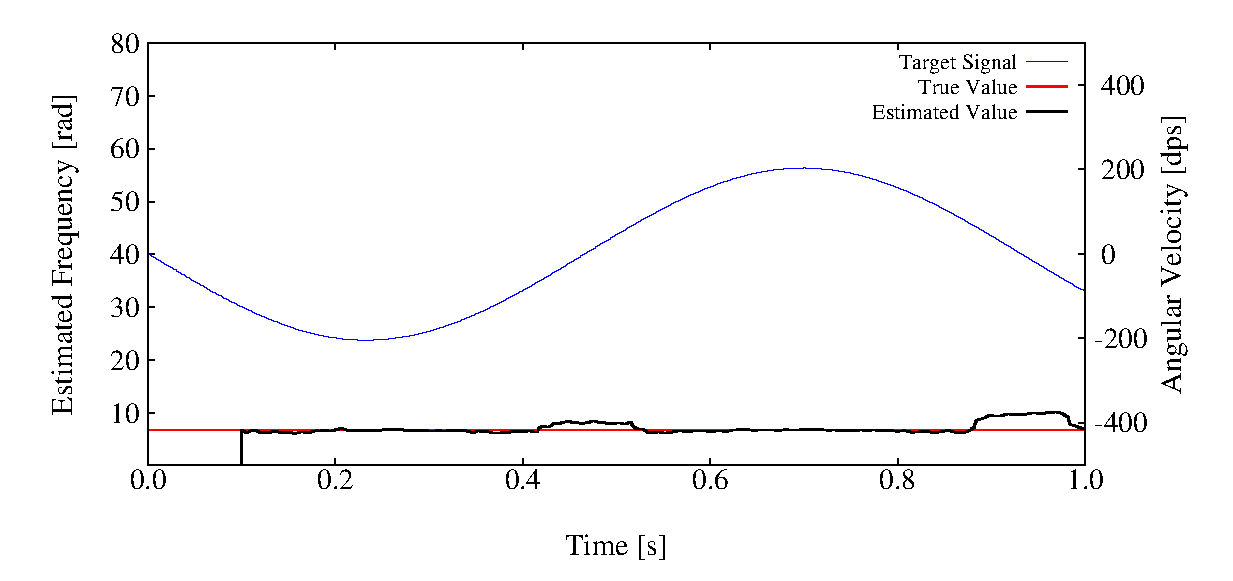
\includegraphics[scale=0.72]{1000hz100.eps}
%     \caption{1000Hz, N=100}
% \end{figure}

% \clearpage
% \samepage
% \begin{figure}[htbp]
%     \centering
%         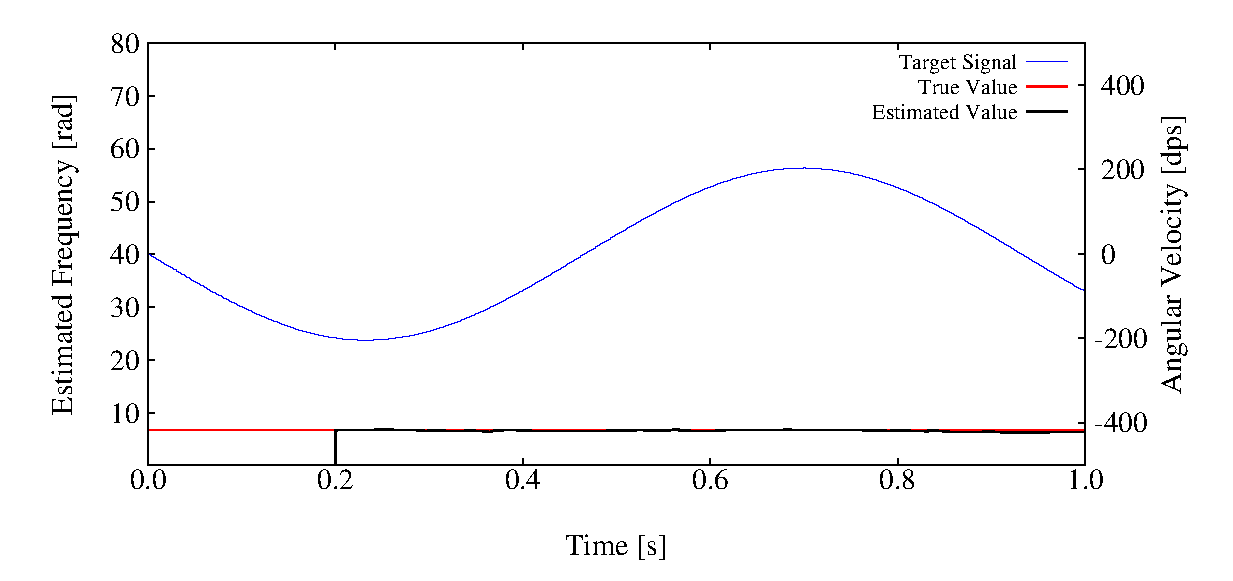
\includegraphics[scale=0.72]{1000hz200.eps}
%     \caption{1000Hz, N=200}
% 		\label{075122_6Feb15}
% \end{figure}
% 以上の結果から,周波数別の参考にするデータ数の変化による平均二乗誤差の推
% 移を図\ref{110716_6Feb15}〜図\ref{ratio}に示す.
% \begin{figure}[b]
%     \centering
%         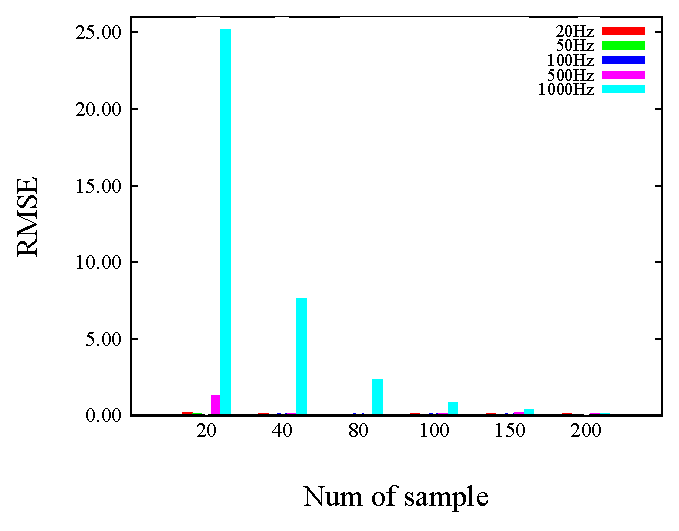
\includegraphics[scale=1]{20_1000rmsebar.eps}
%     \caption{20Hz〜1000Hzの平均二乗誤差の推移}
% 		\label{110716_6Feb15}
% \end{figure}
% \samepage
% \begin{figure}[htbp]
%     \centering
%         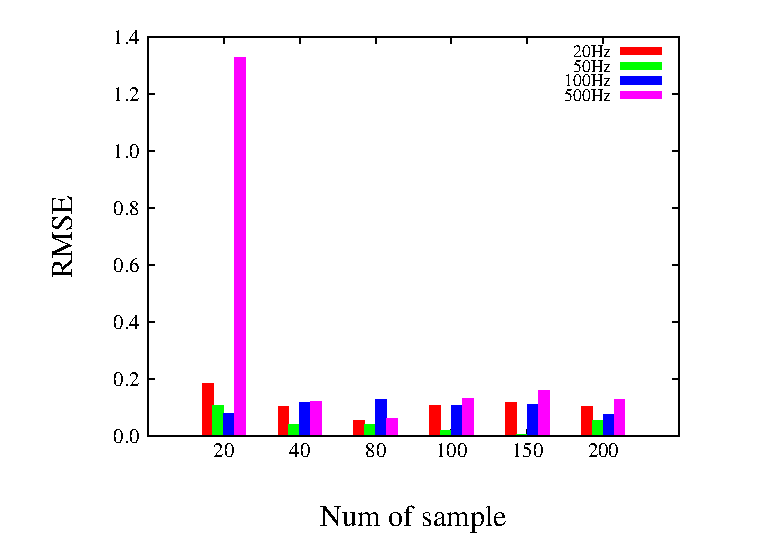
\includegraphics[scale=1]{20_500rmsebar.eps}
%     \caption{20Hz〜500Hzの平均二乗誤差の推移}
% 		\label{012436_7Feb15}
% \end{figure}
% \begin{figure}[htbp]
%     \centering
%         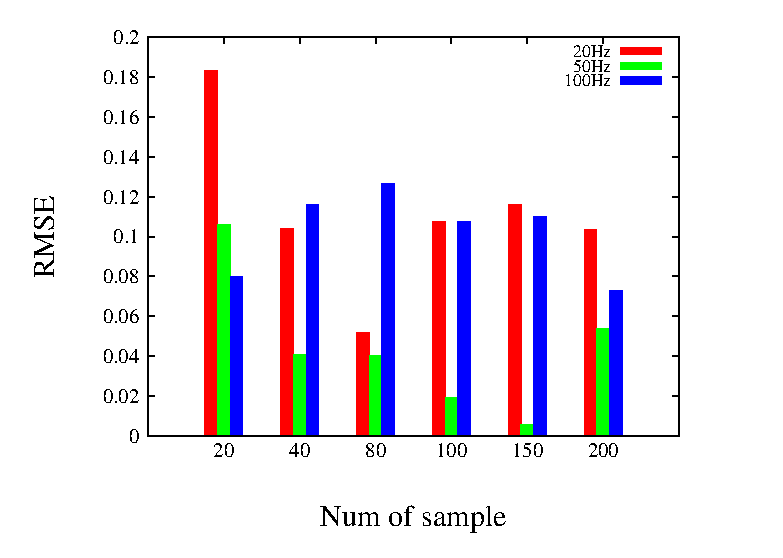
\includegraphics[scale=1]{20_100rmsebar.eps}
%     \caption{20Hz,50Hz,100Hzの平均二乗誤差の推移}
% 		\label{110728_6Feb15}
% \end{figure}
% \samepage
% \clearpage
% \begin{figure}[t]
%     \centering
%         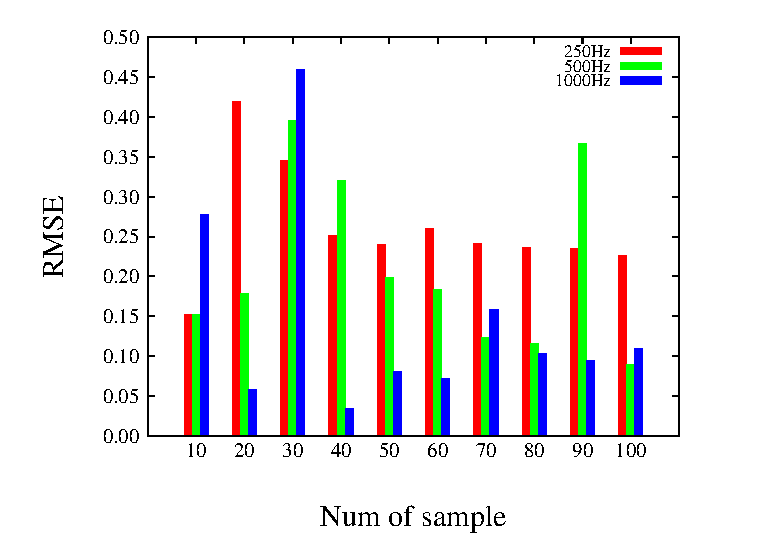
\includegraphics[scale=1]{rmseratiobar.eps}
%     \caption{推定に利用するデータの範囲が占める割合と平均二乗誤差の推移}
% 		\label{ratio}
% \end{figure}

% 図\ref{110716_6Feb15}より,推定に利用するデータ数が20,40,60
% の場合は精度が他の周波数と比較して著しく低下する.これは,周波数を推定す
% るのに振動に関する情報が少ない(1/50周期,1/25周期,3/50周期程度),また,
% 高周波数のためにノイズに影響されやすいことが理由であると考えられる.\\
%  図\ref{012436_7Feb15}では,500HzのN=20のときの誤差は他の周波数に比べ
% 約7倍と大きいが,N=40以上で平均二乗誤差が0.4以内であることがわかる.また,N=200のときに
% 再び誤差が増加している.これは図\ref{020210_7Feb15}で顕著であるが,推定
% する信号の値が0に近づくことで推定値にスパイクノイズが発生するため,参考
% にする信号データによっては精度が安定しない.真値と思われる推定値をノイズ
% と判別することが現段階での課題である.\\
%  図\ref{110728_6Feb15}から,20Hz,50Hz,100Hzの二乗平均誤差は,いずれも0.2
% 以内に抑えられている.参考にするデータ数によって推定精度にばらつきがある
% のは上述した理由と同様に推定値のスパイクノイズであると考えられる.
%  図\ref{ratio}より,まずどの割合においても平均二乗誤差の差は0.5以内に抑
% えられていることがわかる.また3パターンの周波数を比較すると,精度は平均する
% と1000Hz,500Hz,250Hzの順に良ことがわかる.これは,1周期に対して参考にするデータが占
% める割合が同じであっても,データの密度が高いほうが多く情報を参考にできるため
% であると考えられる.また,1000Hzの3/10周期や500Hzの9/10周期を参考にした
% 場合に大きく精度が低下しているのは,上述したように高周波数のためノイズに
% 影響されやすいためであると考えられる.
% \section{まとめ}
% 本論文では超関数を用いた高速周波数推定法を実験的に検証し,以下のことを示し
% た.\\
%  周波数を推定する上で参考にするデータは密度が高く,数が多いほど精度は向
% 上する.しかし密度が高い分だけノイズには敏感である.本論文の検証では推定する振
% 動の1/4周期を参考にし,二乗平均誤差が0.1程度の精度で推定することができた.\\
%  今後の発展として,推定する振動の値が0に近づくことによるノイズの低減や,
% ノイズを含む推定値から真値に近い値を判別する手法の提案等が挙げられる.
\newpage

\section{まとめ}
本論文では,振り子の単振動に対して超関数に基づく周波数推定法を用いて周波数を推定し,以下のことを示した.

超関数に基づく周波数推定をシミュレーションによって検証した.
その結果,量子化ノイズが発生する原因を究明し,提案手法手法1, 2によって量
子化誤差を修正できる
ことを示した.しかし,それぞれの提案手法には長所,短所があり,有効性は推
定するサンプリング周波数やサンプリングデータ数による.

実験では提案手法1, 2によって推定誤差を修正することができ,本手法が有効で
あることを示した.

今後の発展として,振動の周波数が観測中に変化した場合,推定精度を保って追従すること
が挙げられる.また,観測ノイズに推定値が大きな影響を受けるため,適切なフィ
ルタリングを施すなど,精度を向上させる工夫が必要である.
さらに,サンプリング周期とサンプリングデータ数の関係から,最も
精度よく周波数が推定できる関係を考察することを今後の課題としたい.

% 謝辞
\section*{謝辞}
本論文作成にあたり御指導下さった九州工業大学大学院工学研究院機械知能工学
研究系知能制御工学部門西田准教授に深く感謝致します.
さらに,日頃より御協力頂いた機械知能工学科制御工学教室の教職員の皆様
ならびに,同教室西田研究室の皆様に感謝致します.
\newpage
\begin{thebibliography}{99}
\bibitem{fourier} 加藤正昭,``ディジタルフーリエ解析(I)-基礎編-'',コロ
				ナ社,1996.
\bibitem{digital} 加藤幸雄,堤一男,三好正純,清田公保,広林茂樹,``入門ディジタル信号処理'',培風館,pp.85--94,2006.
\bibitem{sf}
 A. Ishizaka, M. Nitta, K. Koto, ``Error analysis on
	 distribution-based frequency estimator'', Proc. of
	 Int. Conf. on Control, automation, and Systems, pp. 255--260, 2010.
\bibitem{distributions} 棚橋隆彦,``エンジニアのための超関数'',三恵社,pp.5--6,2004.
\bibitem{gaus} チャールズ・K・チュウイ,``ウェーブレット入門'',東京電機
				大学出版局,pp.59-60,1999.
 \bibitem{Ni} 新田益大, ``超関数に基づく高精度周波数推定'', 第12回計測自
	 動制御学会制御部門大会, 2012.
\bibitem{omega} 加藤正昭,``物理学の基礎'',サイエンス社,pp.104--105,1996.
\bibitem{toukei} E.クライツィグ,``確率と統計'',培風館,pp.50--51,2010.
\end{thebibliography}

\end{document}
